\documentclass[11pt]{article}

\usepackage{common}
\usepackage{booktabs}
\usepackage[margin=1in]{geometry}
\usepackage{hyperref}
\title{The Analytics Edge, Final Report:\\ Building a Topic Model as First Steps Toward an Article Recommender for Bleacher Report Basketball}
\author{for Professor Dimitris Bertsimas and Emma Gibson \text{ } \\ \\ by Stephen Albro \& Cyrille Combettes \\ salbro@mit.edu, cyrille@mit.edu}
\begin{document}
\maketitle{}


\section{Motivation and Project Abstract}
In an age of cut-throat digital competition, it is vital for websites to be able to retain visitors to compete for advertising revenue. Bleacher Report, a primary digital destination for sports article readers, contains well written articles covering the league, and competes as advertisement real-estate with the likes of ESPN.com and others. Bleacher Report hopes for two things from each visitor. First, \textit{prolonged} visitors: that the visitor spend a lot of time on the website, jumping from article to article.  Second, \textit{frequent} visits: that the visitor develops a loyalty to the website.  We feel that having a micro targeted article recommendation system would help Bleacher Report foster long visits and loyalty among its consumer base, and thus provide an analytics-based edge over its competitors.  

In order to recommend articles, it is necessary to express those articles mathematically. In particular, we seek a good \textit{embedding} of each article in an appropriate vector space.  A reasonable document-recommendation strategy is to then, using visitor's history, recommend Nearest Neighbors within that space. Our project focuses on exploring such an article-embedding strategy based on \textit{topics} found in the article corpus. This strategy is known as \textit{Topic Modeling}, and within that, we took an approach known as \textit{Latent Dirichlet Allocation (LDA)}.  

We note briefly that we determined LDA to be the most promising of three approaches to this problem by doing an initial experiment which also included two other approaches: word2vec title embeddings, and Non-Negative Matrix Factorization (NMF) topic modeling. This initial experiment can be found in the Appendix.

\section{Data Collection}
Bleacher Report does not provide database access to their articles.  However, News API is a company that provides API access to news metadata, including URLs, from a variety of sources, including Bleacher Report.  Using NewsAPI, we queried Bleacher Report NBA articles from October 17, the start of the 2017-2018 NBA season. Our entire query consisted of joining words like basketball and NBA with all 30 teams and the top 25 active players.  In the end, we received 3314 URLs (with their corresponding authors, titles, and other metadata) in return.  We then scraped the content of each Bleacher Report article URL. 

\section{Data Cleaning}
In the real world, data is never clean, but text data is as messy as it gets. There were a number of preprocessing steps we had to do before our articles were ready for analysis. In our cleaning efforts, we made decisions with our ultimate goal in mind, which was to find a good embedding for our articles based on topics.  Because of this, a bag-of-words cleaning mindset was chosen over one that preserved grammar.

%\subsubsection{Punctuation Removal, Initial Stopwords, and Lowercasing}
First, we tokenized each article. In natural language processing, tokenizing is a way of chopping up a document into pieces, the most obvious way being to tokenize by \textit{word}, which is what we initially did.  We discarded any non-alphabetical tokens (e.g. 8pm, 704, !, .), and converted everything to lower case.  Then, we removed 170 basic \textit{stop-words}, such as \textit{a, the, his}, and \textit{my}. 

%Then, we did our first round of stop word removal.  In  NLP a stop word is any word that you remove because its insignificant for your application.  In this first round, we removed basic articles (the, a) and about 170 other words deemed insignificant by Python's Natural Language Toolkit, mostly personal pronouns and simple verbs.

%\subsubsection{Specialized NBA Tokenization}
Next, we needed to somehow tokenize important entities in our corpus, such as players, teams, and coaches. The reason for this is that each player, for example, can be referred to in a variety of ways. For example, the NBA superstar LeBron James can be called LeBron James, LeBron, Bron, or James. Similarly, the Boston Celtics might be formally referred to as such in the title, but in the article's body they might just be Boston. For each article, we replaced all forms of each entity with an underscored and fuller version, so that, for example, LeBron James would always be lebron\_james, no matter if he occurred as Bron, James, or Lebron in a given sentence.  At times it was necessary to infer from ambiguous usage. We concluded that, for example, the word \textit{Boston} should be replaced by boston\_celtics only if the entire phrase Boston Celtics appeared somewhere in the article.  This specialized, application-specific tokenization step would allow us to capture much more contextual information about each superstar, team, and coach.

%\subsubsection{Stemming Each Word}
Next, we \textit{stemmed}. Stemming addresses the fact that the root of a word (e.g. \textit{play}) can take different grammatical forms (\textit{playing, played, plays}). As far as topic modeling goes, it makes sense to make a stemming simplification. We used Python's Natural Language Toolkit stemmer.

%\subsubsection{Trimming Down the Vocabulary}
Finally, and perhaps most importantly, we significantly reduced the size of our vocabulary. In NLP, a \textit{vocabulary} is simply the complete set of words that the model knows about.  Since we were modeling topics, we thought it would be important to feed the model information-containing words (player and team names, high-impact verbs, league terminology), and remove all mundane nouns and verbs from our articles (essentially expanding our set of stop-words). 

To choose the words in our vocabulary, we used a \textit{document frequency} approach. The document frequency of a given word is simply the fraction of documents (articles) in which the word appears. The word \textit{the}, for example, has a document frequency of 1.0. If a word occurs too \textit{infrequently}, it is probably a unique name or an article-specific entity, and thus unhelpful from a topical standpoint. On the other hand, if a word occurs too \textit{frequently}, it is probably a common word and thus also contains very little topic information.

Therefore we sought lower and upper document-frequency cutoff thresholds as a way of narrowing our vocabulary.  We knew the upper threshold had to be at least high than the document frequency of LeBron James (0.22, he the most famous superstar), since every player should be in the vocabulary. After seeing irrelevant words persist with even an upper threshold of 0.5, we knew that the upper cutoff had to be lower than that. After eye-test experimentation we decided upon 0.23. Our lower cutoff was 0.01, which means that if a word appeared in less than 34 out of 3314 total articles, it was discarded.

The new vocabulary consisted of about 3500 tokens with document frequencies within the range (0.01, 0.23), including the major players and teams, and important information-containing sports and NBA terminology.  To give a sense, the first few printed tokens are \textit{fewest, monday, march, eric\_bledso, toronto, decid, blowout, jae\_crowd,} and \textit{aggress}.  

\section{Topic Modeling with Latent Dirichlet Allocation}
As we have been saying, it is necessary to embed articles in some vector space in order to produce neighbor-based recommendations. In this section we introduce and discuss the training and tuning of our final LDA topic model. We explore its results with insightful visualizations of the Bleacher Report topic landscape, and do one final sanity-check of our model by clustering articles based on their topical composition. 

\subsection{Introduction to Topic Modeling and LDA}
In the following section, let \\
$D = \{d_1, d_2, ... d_N \}, \quad$ the set of $N$ documents (articles) obtained from Bleacher Report \\
$V = \{w_1, w_2, ... w_M \}, \quad$ the set of $M$ words in the final vocabulary \\
$T = \{t_1, t_2, ..., t_K\}, \quad$ the set of $K$ topics in the documents 

In topic modeling, we attempt to infer which \textit{topics} are present among the documents, and then after that, to identify which topics belong to each particular document, and in what proportion.  A \textit{topic} is defined as a frequency distribution over all words in the vocabulary.  For each topic, each word has a probability of being chosen.  The task is difficult, because we are trying \textit{both} to infer the topics themselves (all we provide in advance is $K$, the number of topics), \textit{as well as} the topic-composition of each document.

We decided upon a specific Topic Model known as Latent Dirichlet Allocation (LDA). LDA is a bag-of-words model, as opposed to one that considers grammar.  It assumes that each document is created according to the following generative process: \\
$\text{} \quad$ 1. Randomly generate a distribution over topics\footnote{This requires a distribution over a distribution. The  topic distribution is assumed to have a Dirichlet prior, giving the model its name}. \\
$\text{} \quad$ 2. To come up with each word in the document: \\
$\text{} \quad$ $\quad$ a. Randomly choose a topic. \\
$\text{} \quad$ $\quad$ b. Randomly choose a word from that topic. 

We provide the number of topics, and then the task of LDA is to infer the following two parameters, by maximizing the likelihood (according to the story of the generative process described above) of the articles in our corpus: \\
$\text{} \quad \beta_t$: the distribution over words for topic $t$: $\mathcal{P}(w | t) \quad \forall w \in V$ \\
$\text{} \quad \theta_{dt}$: the proportion of document $d$ that came from topic $t$: $\mathcal{P}(t | d) \quad \forall t \in T$ 

%%%%%%%%%%%%%%%%%%%%%%% CLEAN STOP %%%%%%%%%%%%%%%%%%%%%%%%%
The fitted model allows us to express each document as a distribution over the topics it is estimated to contain. Thus, we can accomplish our task of \textit{embedding each article as a K-dimensional vector}, which represents its topical makeup.  The vectorized documents can then be clustered based on their topical composition. The idea is that if I love the topic of statistics and I also love the topic of Lebron James, I will be recommended articles about Lebron James' statistics.  

\subsection{Training LDA with Grid Search}
When training the LDA model in Python, two hyper-parameters needed to be fine-tuned. The first was $K$, the number of topics to provide.  The second was $\gamma$, the learning rate of the solver. We decided to use a grid search cross validation approach.  Since topic modeling is an unsupervised problem, there was no need for a separate validation set, nor was there a supervising value.  Instead, we used the log-likelihood of the trained model as our measure of model quality. 

First, we searched $k \in \{10, 15, 20, 25, 30\}$ and $\gamma \in \{.5, .7, .9\}$. On the left are the grid search results, the log likelihoods for each parameter duo. After discovering that the best hyper-parameters were found to be $k=10$, $\gamma = 0.7$, we decided to narrow down the grid search further (right) to find the absolute best number of topics.  After searching over $k \in \{10, 11, 12, 13, 14\}$ and $\gamma \in \{.5, .7, .9\}$, we moved forward with the optimal $k=13$ topics (and $\gamma = 0.7$). \\

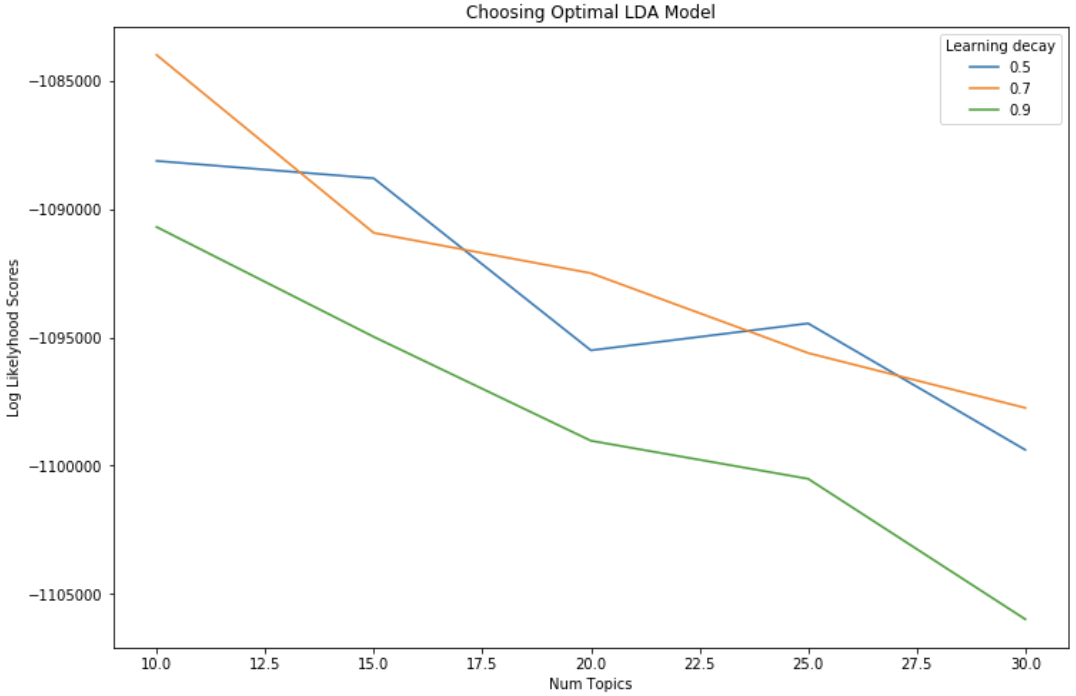
\includegraphics[width=225pt]{gridsearch.png} 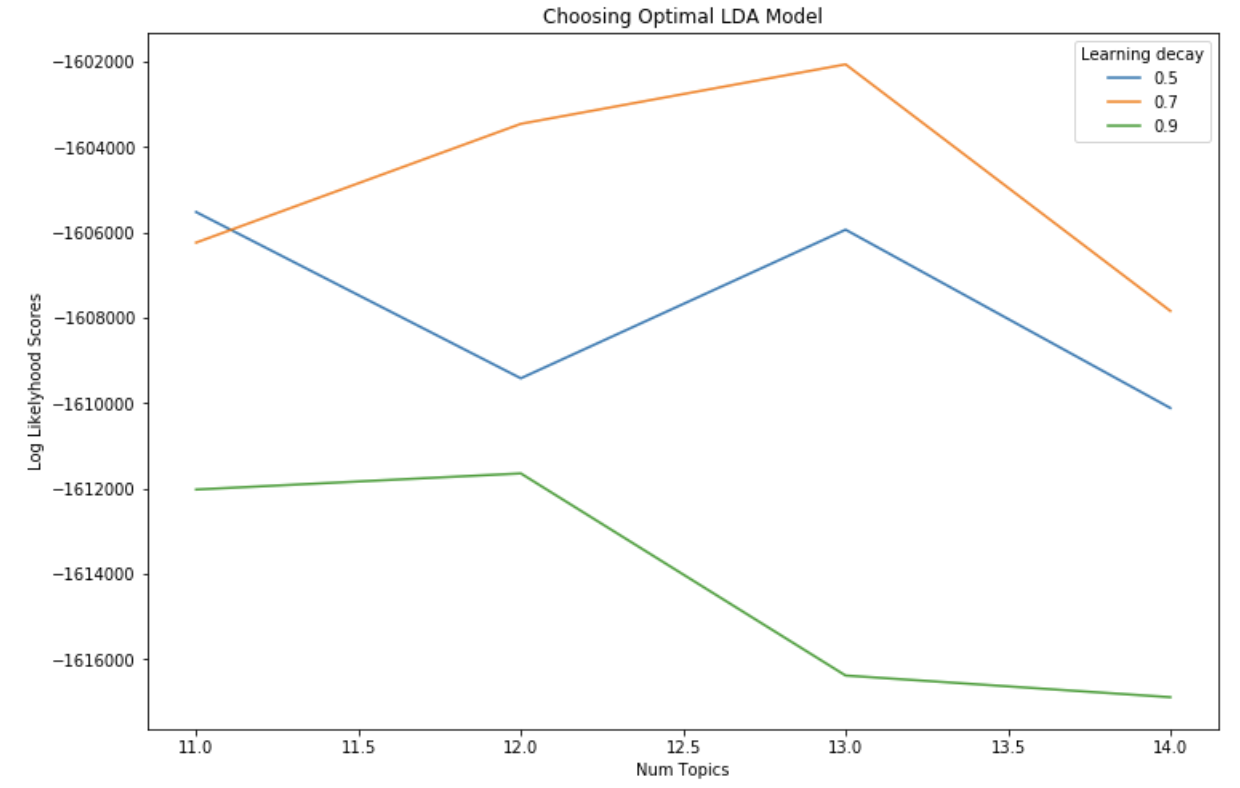
\includegraphics[width=225pt]{gridsearch2.png} 

\subsection{LDA Results}
\subsubsection{Visualization}
As avid NBA fans, we were very pleased to discover that our topics made great sense.  We visualized them using LDAvis, a method for visualizing LDA topics developed by Carson Siever and Kenneth Shirley \footnote{Sievert, Carson and Shirley, Kenneth. "LDAvis: A method for visualizing and interpreting topics". \textit{Proceedings of the Workshop of Interactive Language Learning, Visualization, and Interfaces}, pages 63-70, Baltimore, Maryland, USA, June 27, 2014. Their Github can be found \href{https://github.com/cpsievert/LDAvis}{here}}.  The visualization has two primary components.  On the left, the blue circles represent the topics. The size of each circle represents the proportion of its topic occurance across all documents. The positions of the circles is meant to be a 2D projection of their locations with respect to each other in the topic space. Specifically, a matrix of inter-topic distances is generated, \footnote{Remember that a topic is a probably distribution over all words in the vocabulary. The distance between two topics is found by computing the Jensen-Shannon diveragence between their distribution.}, where each row in the matrix contains one topic's distances to every other topic.  The $K$-dimensional distance rows are then shown in 2 dimensions using Principal Component Analysis \footnote{Though the topics themselves sense, we cannot detect any semantic meaning in the first two principal components.} This visualization technique is known as \textit{multidimensional scaling}, and typically performed on distance matrices as in this case. 

On the right, the red bars indicate the estimated number of times a given term came from a given topic. When you hover over a topic, the 30 most relevant terms from that topic are shown.\footnote{$\text{relevance}(w | t) = p(w | t) + p(w | t)*p(w)$}  Our visualization is interactive, and we recommend that you run it in our notebook, RUNME.ipynb.  However we we show a few topics here. 

The most prevalent topic, 1, is all about player statistics (steals, blocks, defensive and offensive rates, ranks, percentages, etc.). It makes sense that this is the most prevalent topic in a corpus full of sports articles. 

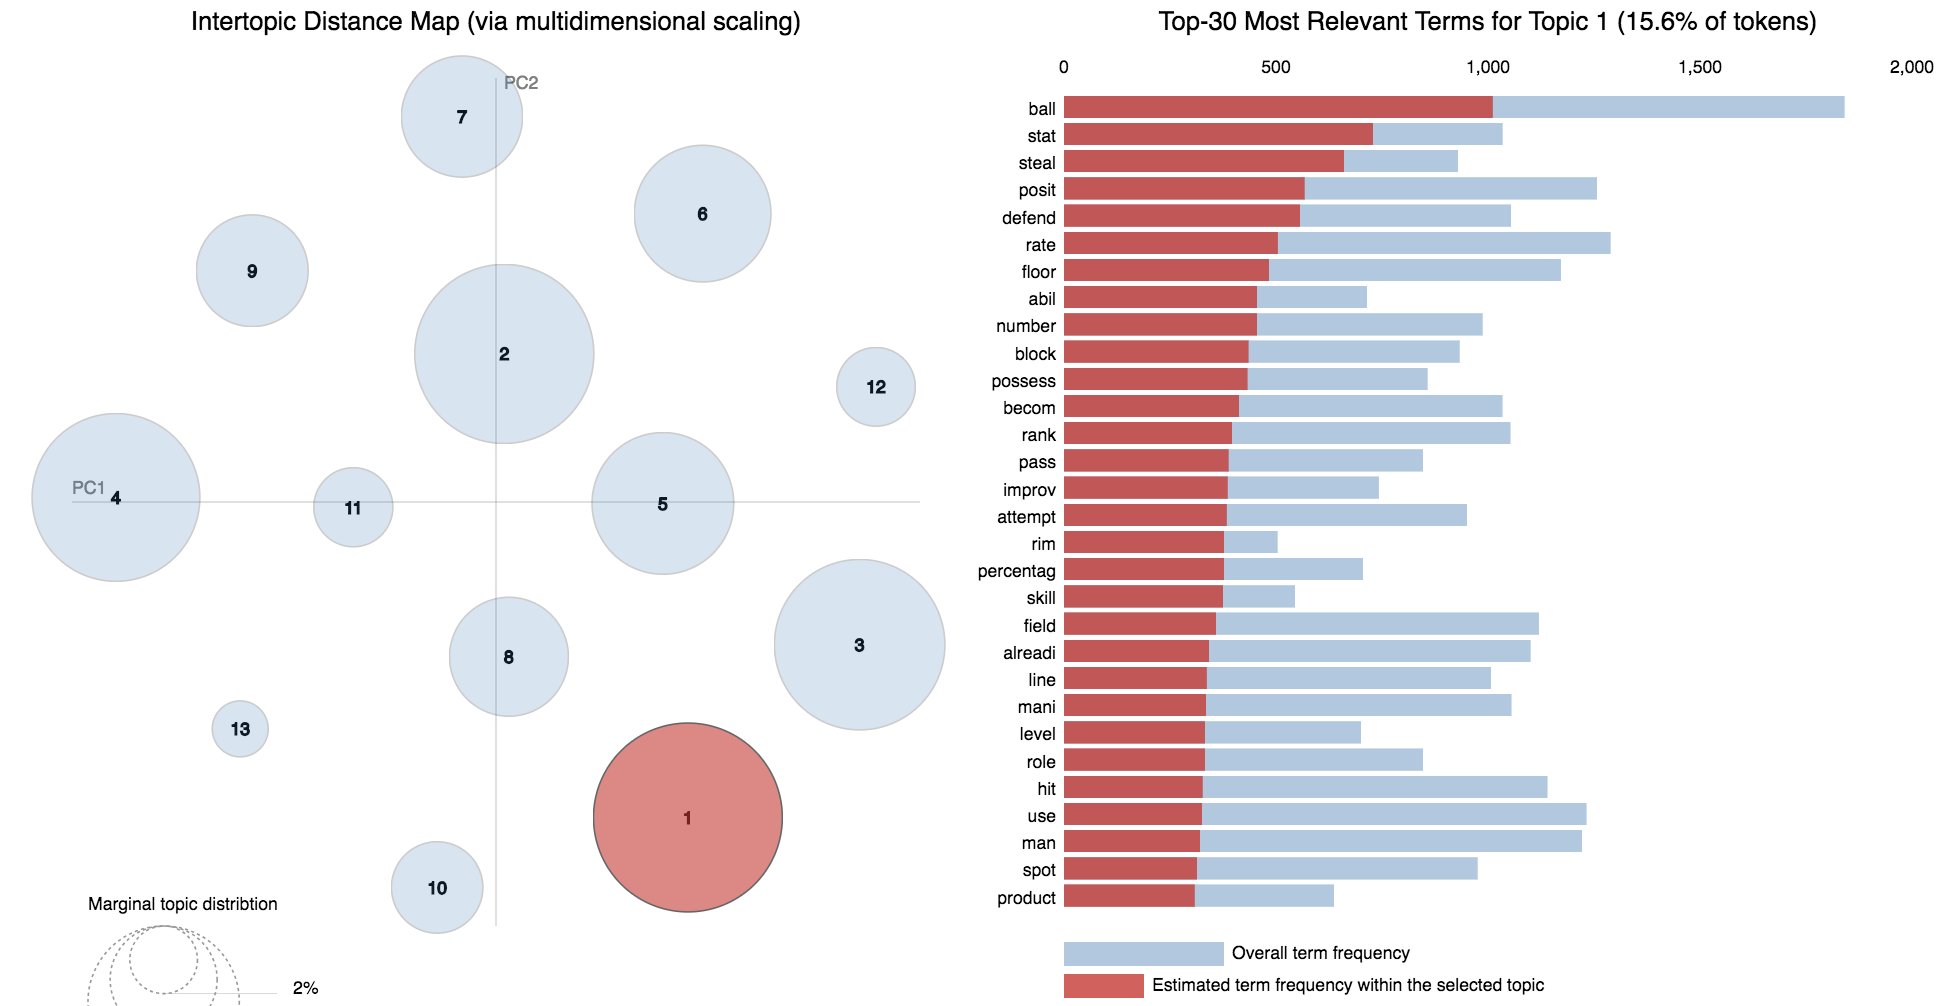
\includegraphics[width=470pt]{1.png} 

To its right, topic 3, seems to be about the Golden State Warriors, the best team in the NBA (mostly because of superstars Stephen Curry and Kevin Durant), and their competition in the Western Conference (including James Harden's Rockets and Russel Westbrook's Thunder). 

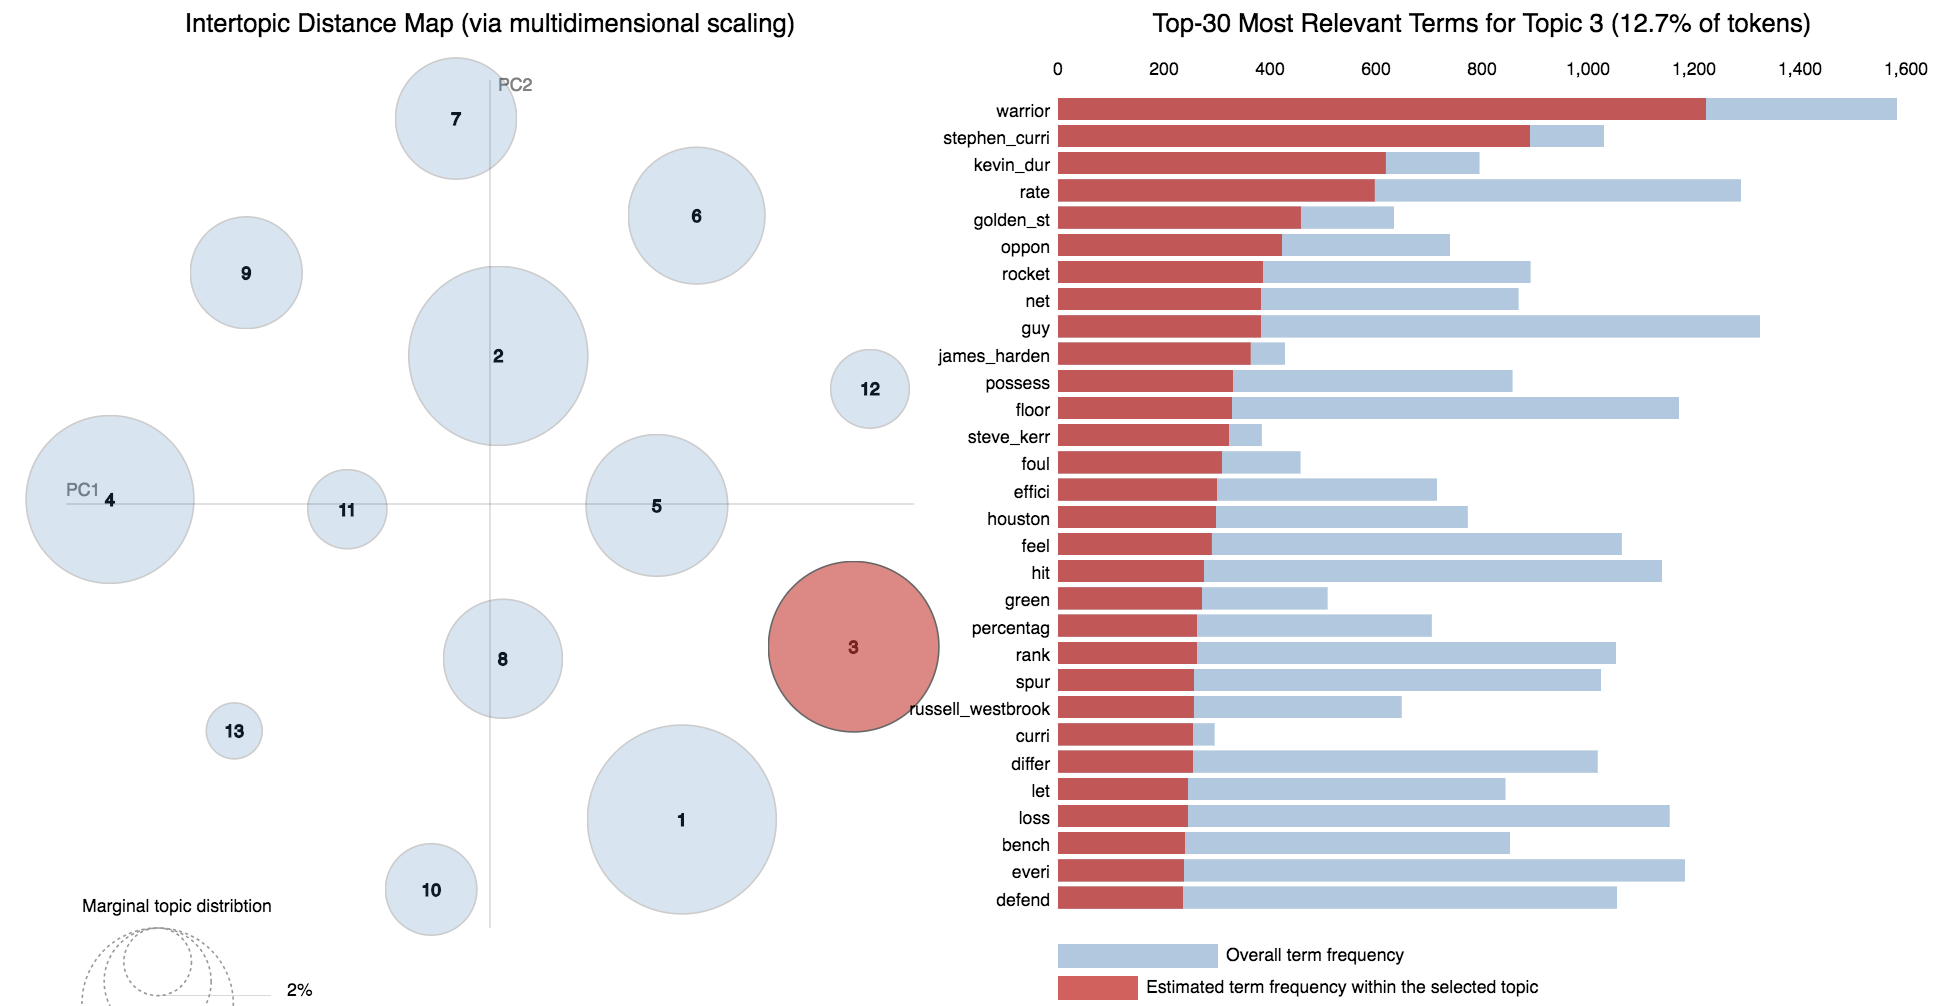
\includegraphics[width=470pt]{3.png} 

Topic 4 is all about the economics of the NBA, including trade deals, free agency signing decisions, and salary information.

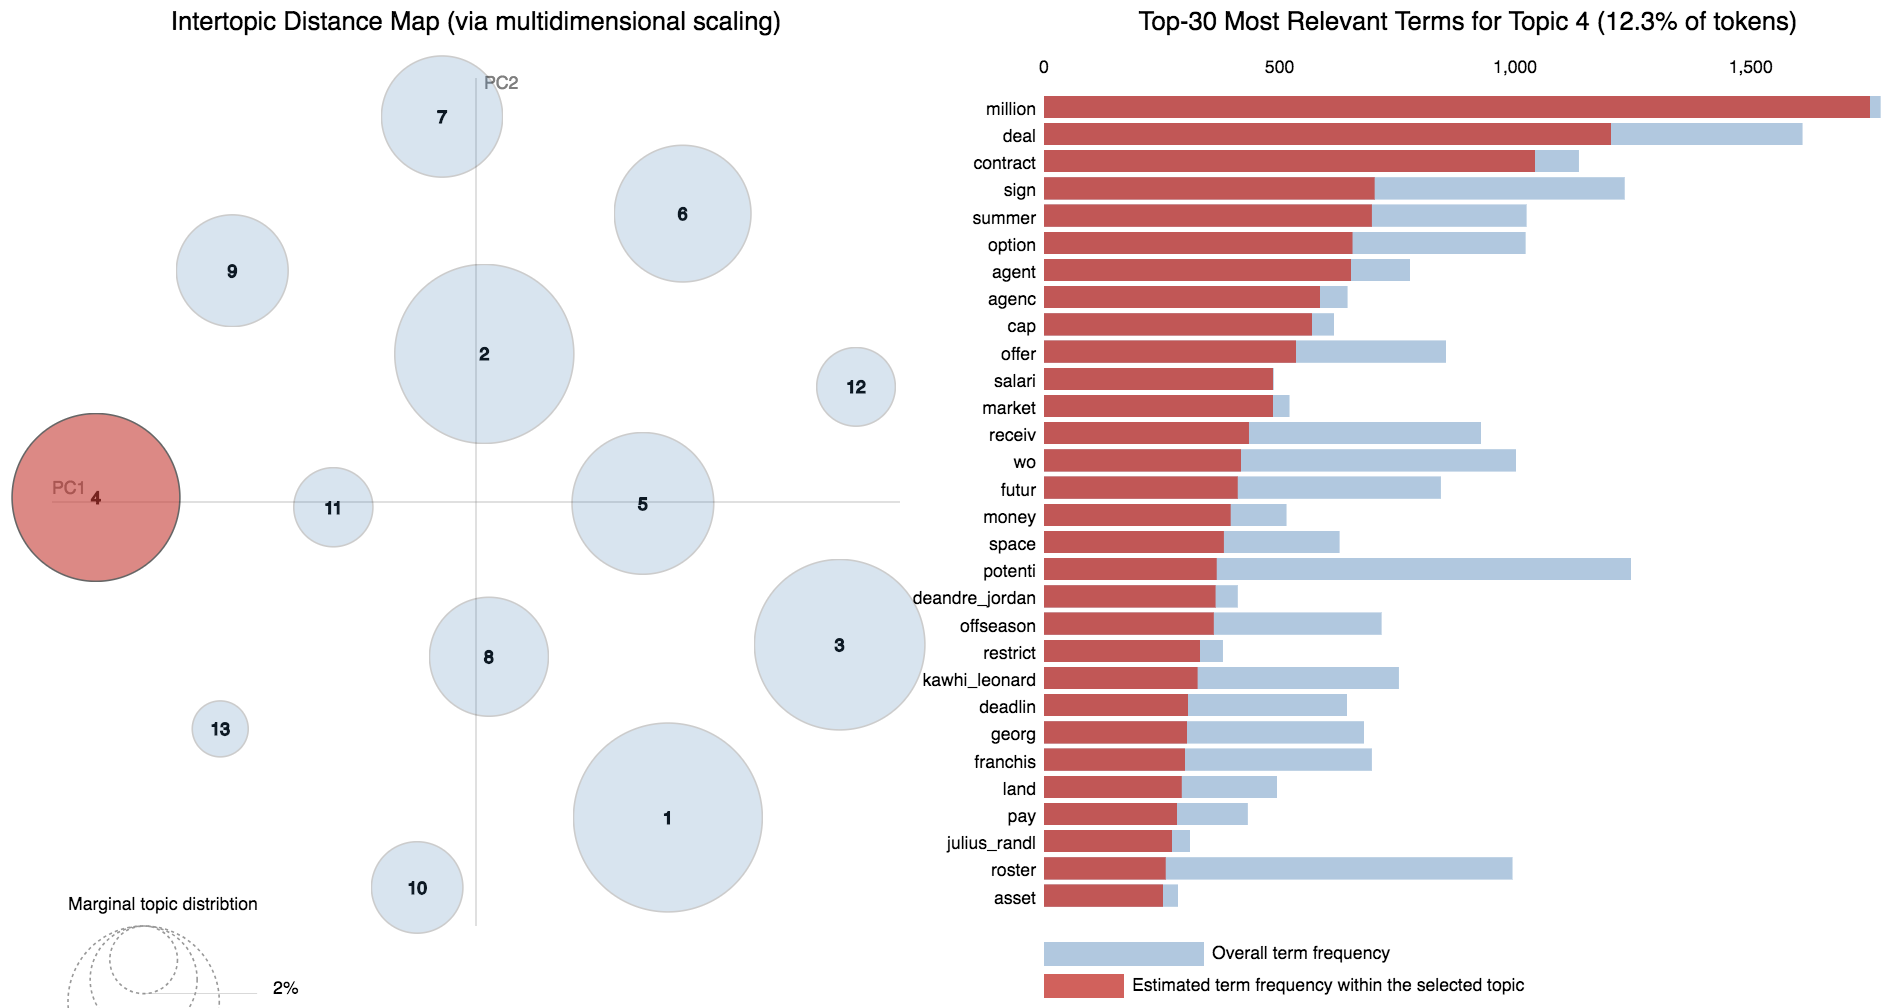
\includegraphics[width=470pt]{4.png} 

Topic 5 is our personal favorite, as it is all about Lebron James.  The most salient words in topic 5 are Lebron, his team mates, his team name, his coaches, and his major rivals.  

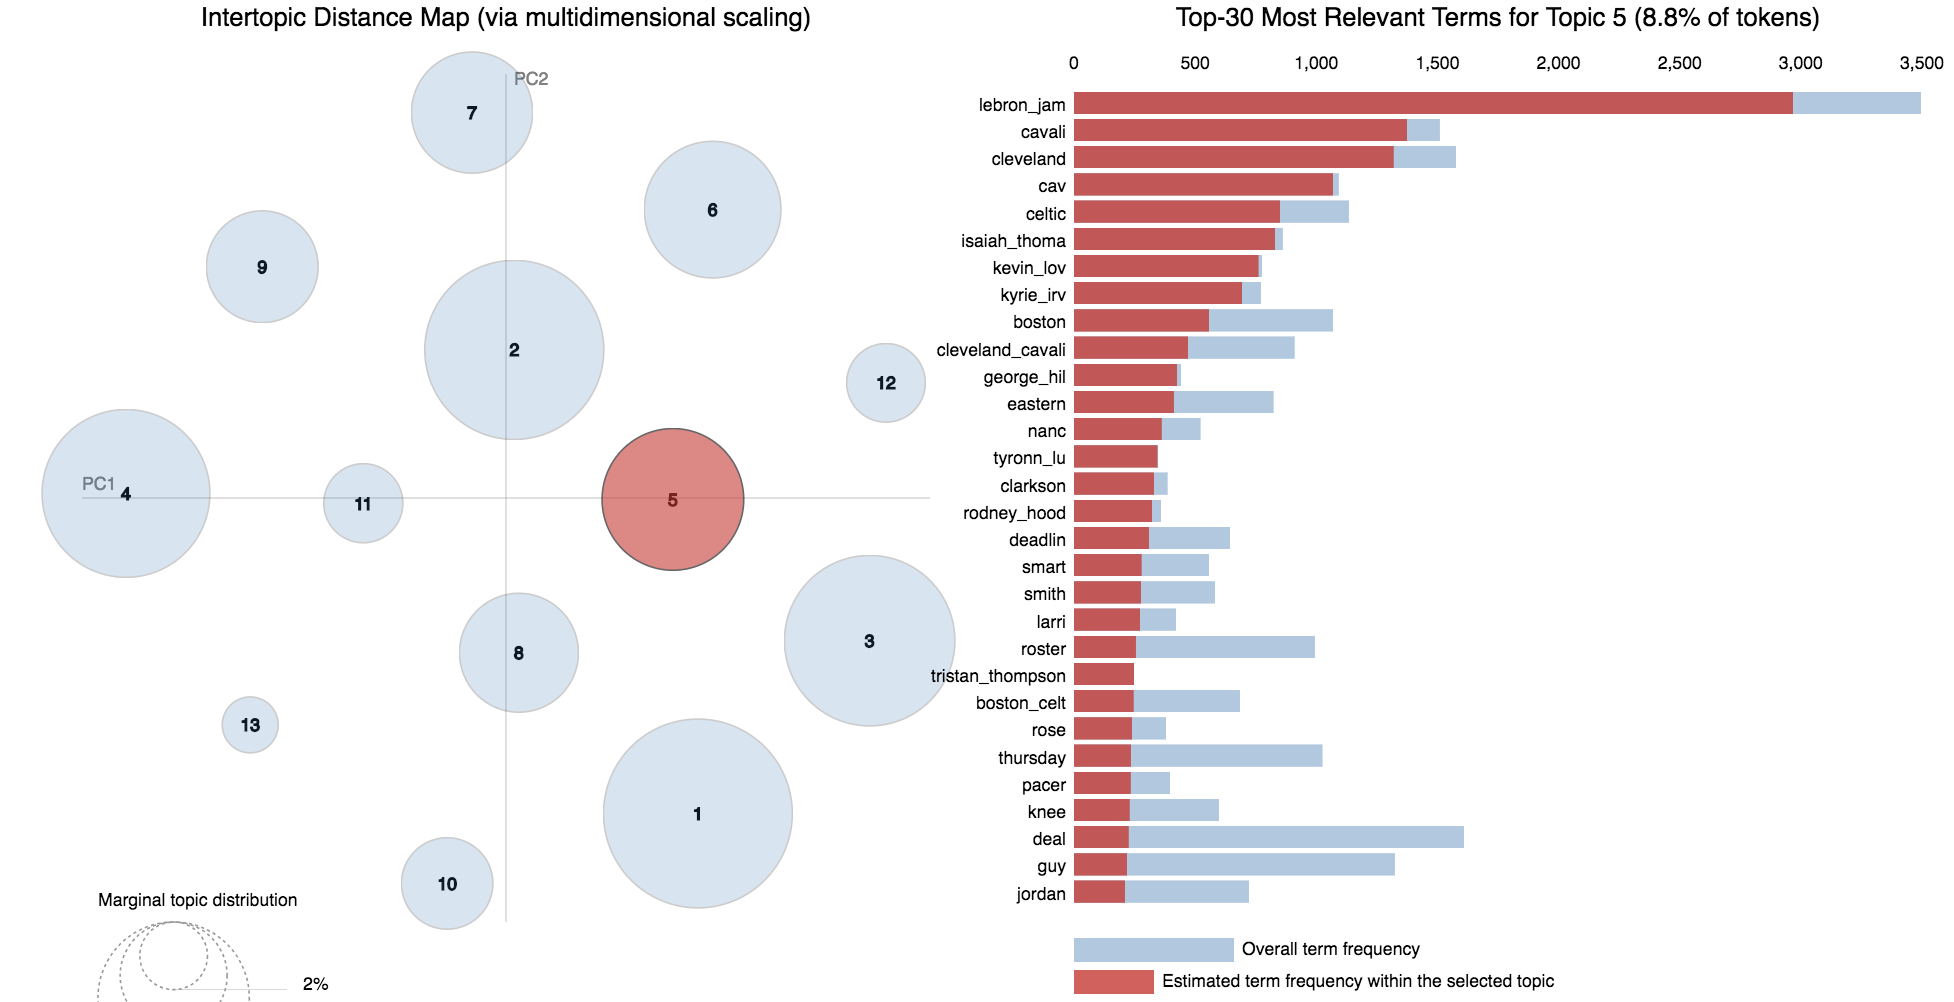
\includegraphics[width=470pt]{5.png} 

In fact, if you hover over the term \textit{lebron\_james}, you can see his primary topics. Topic 5 dominates as his primary topic. 

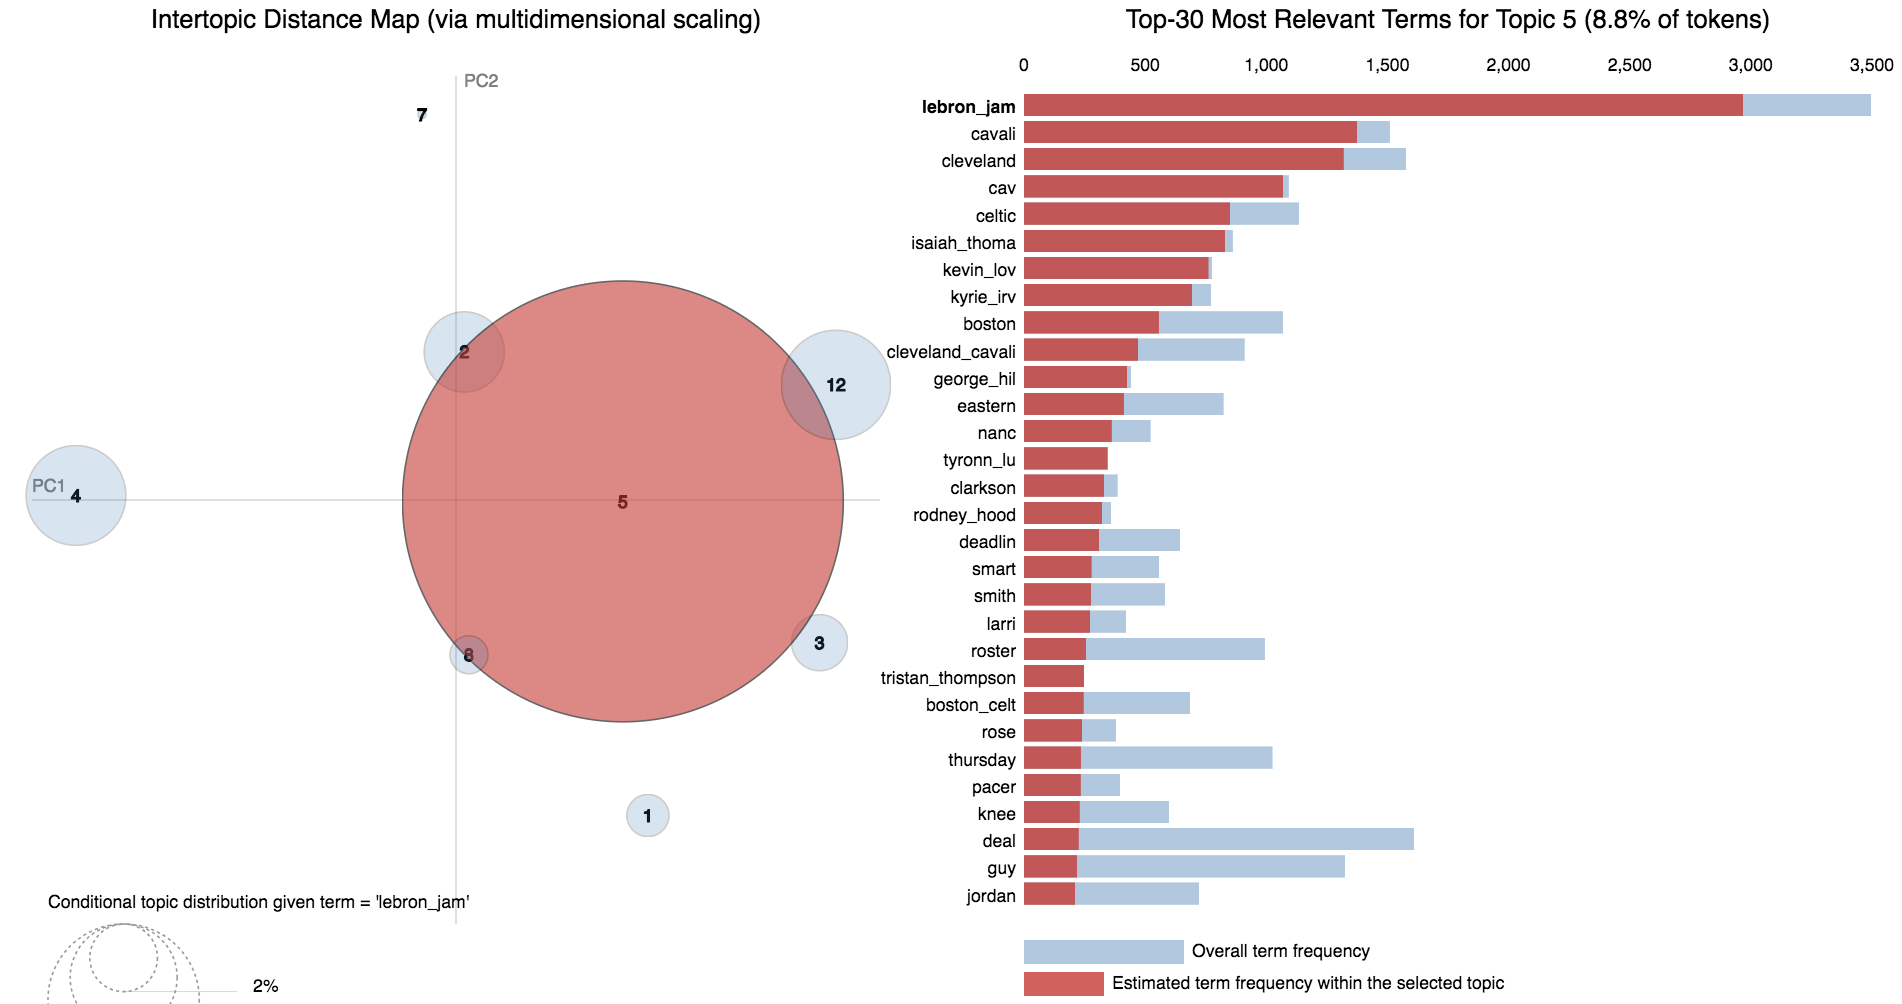
\includegraphics[width=470pt]{6_lebron.png} 


Topic 6 collected the terms pertaining to the NCAA March Madness college basketball tournament, which pushes aside the NBA in popularity for a brief month as the college kids take center stage. Michigan played Villanova for the championship this year. \\
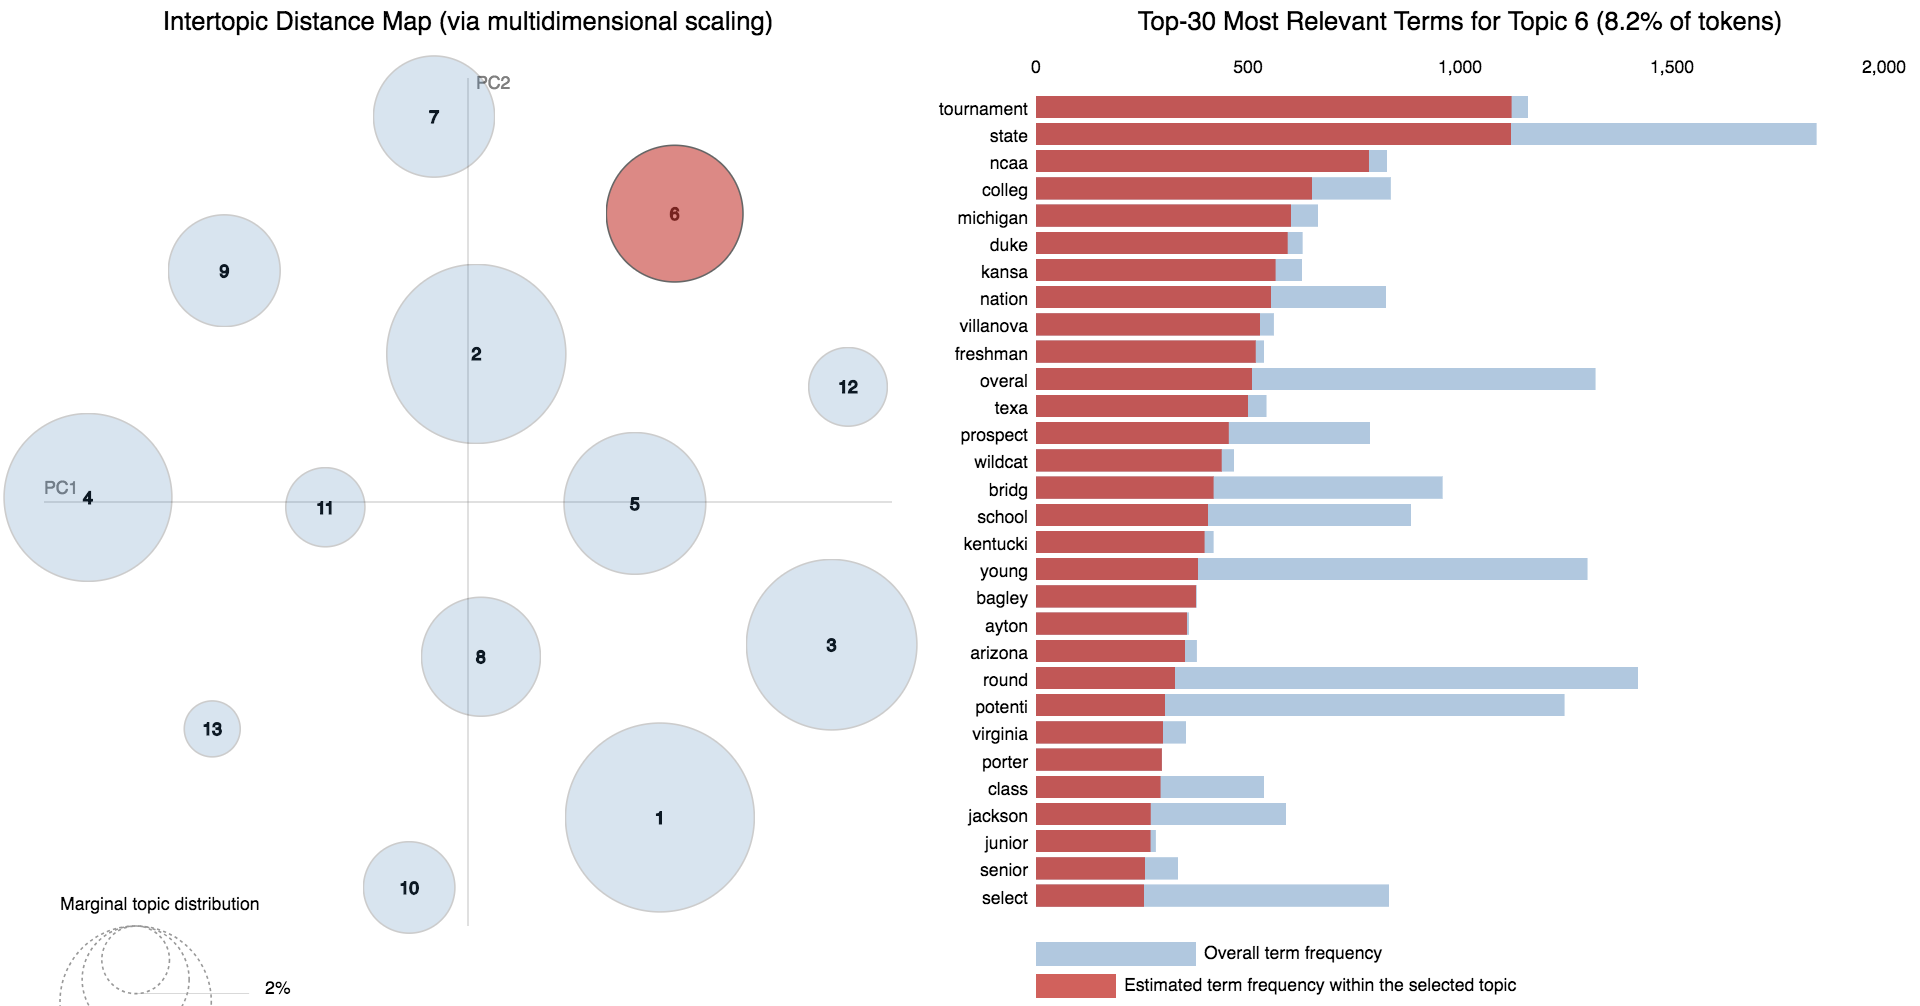
\includegraphics[width=470pt]{6.png} \\

Topic 7 seems to be about the playoffs, seeding, and exciting first-round matchups.  \\
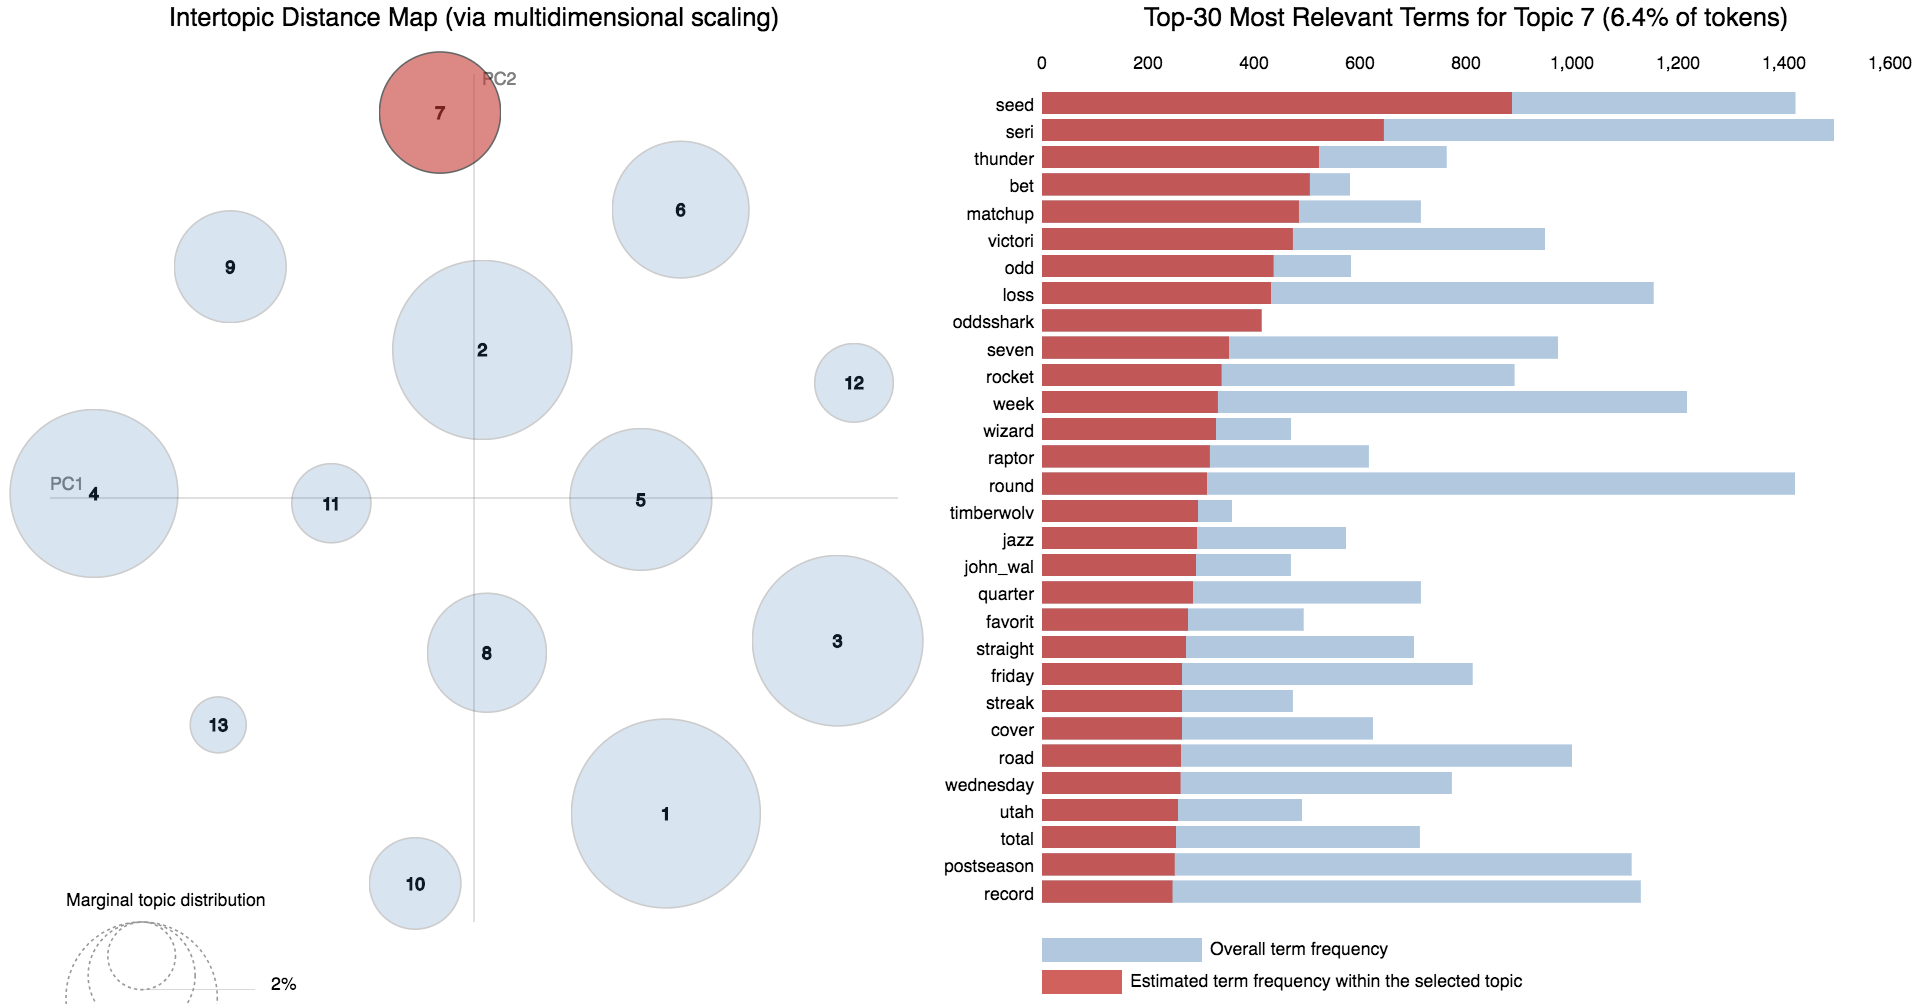
\includegraphics[width=470pt]{7.png} \\

Topic 13 is actually about soccer!  The NewsAPI must have returned a handful of soccer-related articles with the basketball ones, and our LDA model discovered that. \\
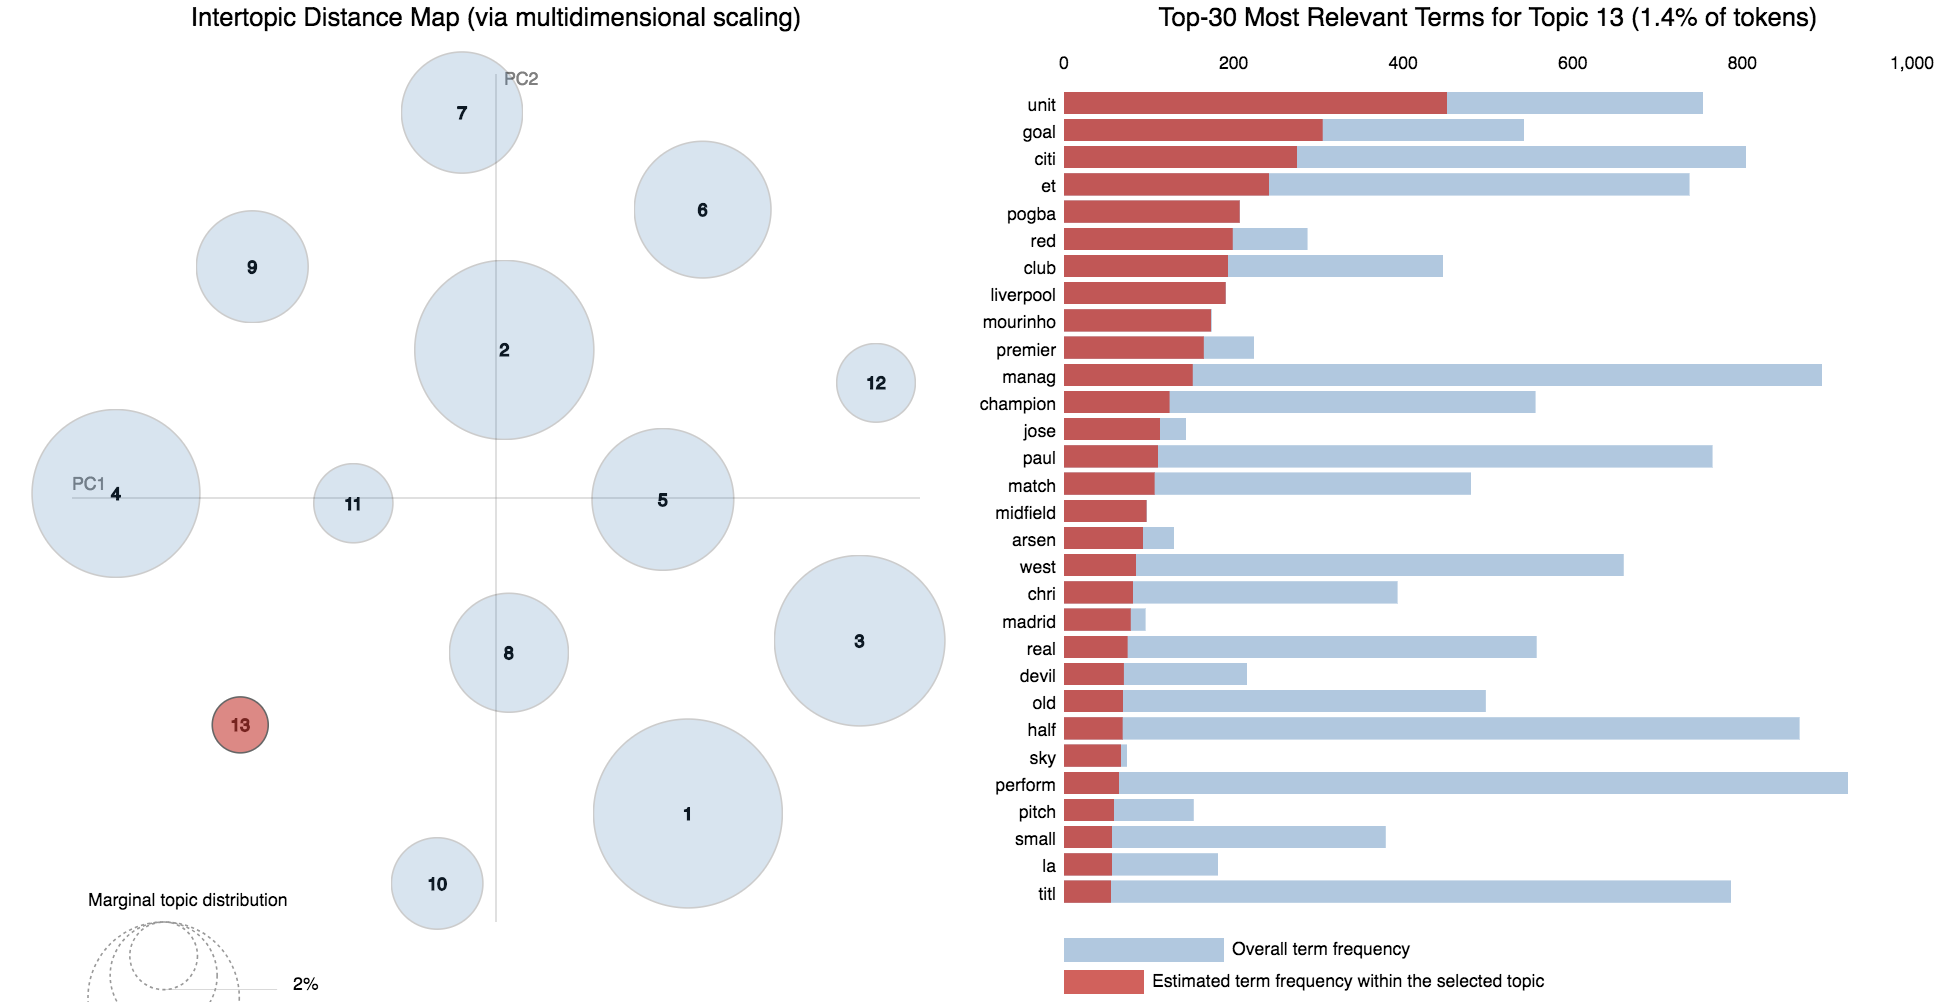
\includegraphics[width=470pt]{13.png} \\

We have left the visualizations of other topics in the appendix, for brevity's sake.

%Finally, in addition to visualizing the topics, we did one final sanity check on the quality of the topics. We vectorized each article by embedding it as a 13-dimensional vector, which represents its estimated topical composition according to the topic model.  At that point we clustered the articles in topic space.  The detail is left for the appendix, but in short, we found that the clusters made reasonable sense. 
\subsubsection{Sanity Checking the Topics by Clustering Articles According to Topical Composition}
We already felt good about the quality of our topics because the visualizations showed them to be cohesive and comprehensive. However, we figured that it could not hurt to cluster the articles in topic space as a final sanity-check.  We used KMedoids for this clustering, which allowed us to specify a custom distance function (KMeans does not necessarily converge for non-Euclidean distances).  Our custom distance function was the Jensen-Shannon divergence metric, which measures the similarity between two probability distributions.  This was appropriate because our articles have been expressed as distributions over topics.  (An alternative method could have been to just assign each article to a cluster of its most prevalent topic.)  Using the "elbow" method, we found that a reasonable number of article clusters was 8. We found this by plotting the total sum of distances to each medoid for various numbers of medoids and then looking for the plateauing elbow point.  \\

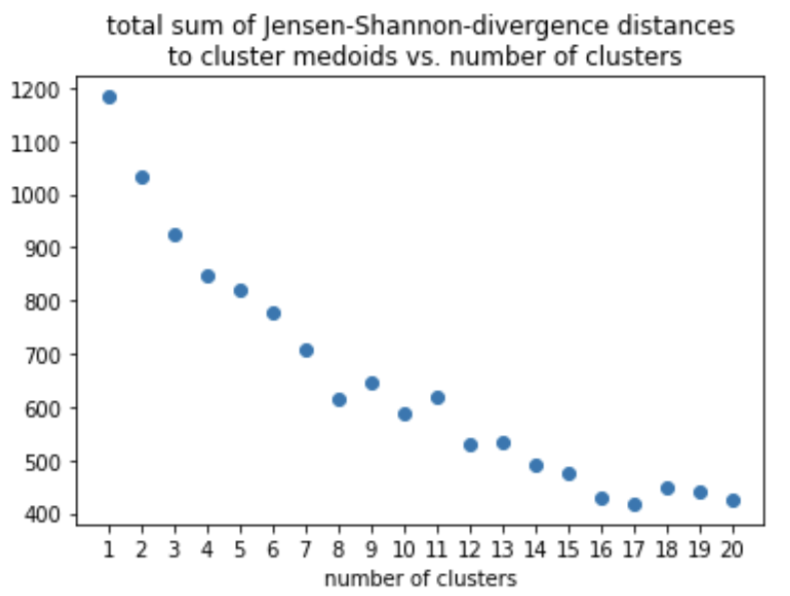
\includegraphics[width=350pt]{jensen.png} \\

Here we plot, coloring by cluster, each article along the two SVD decomposed components from the LDA output matrix. 

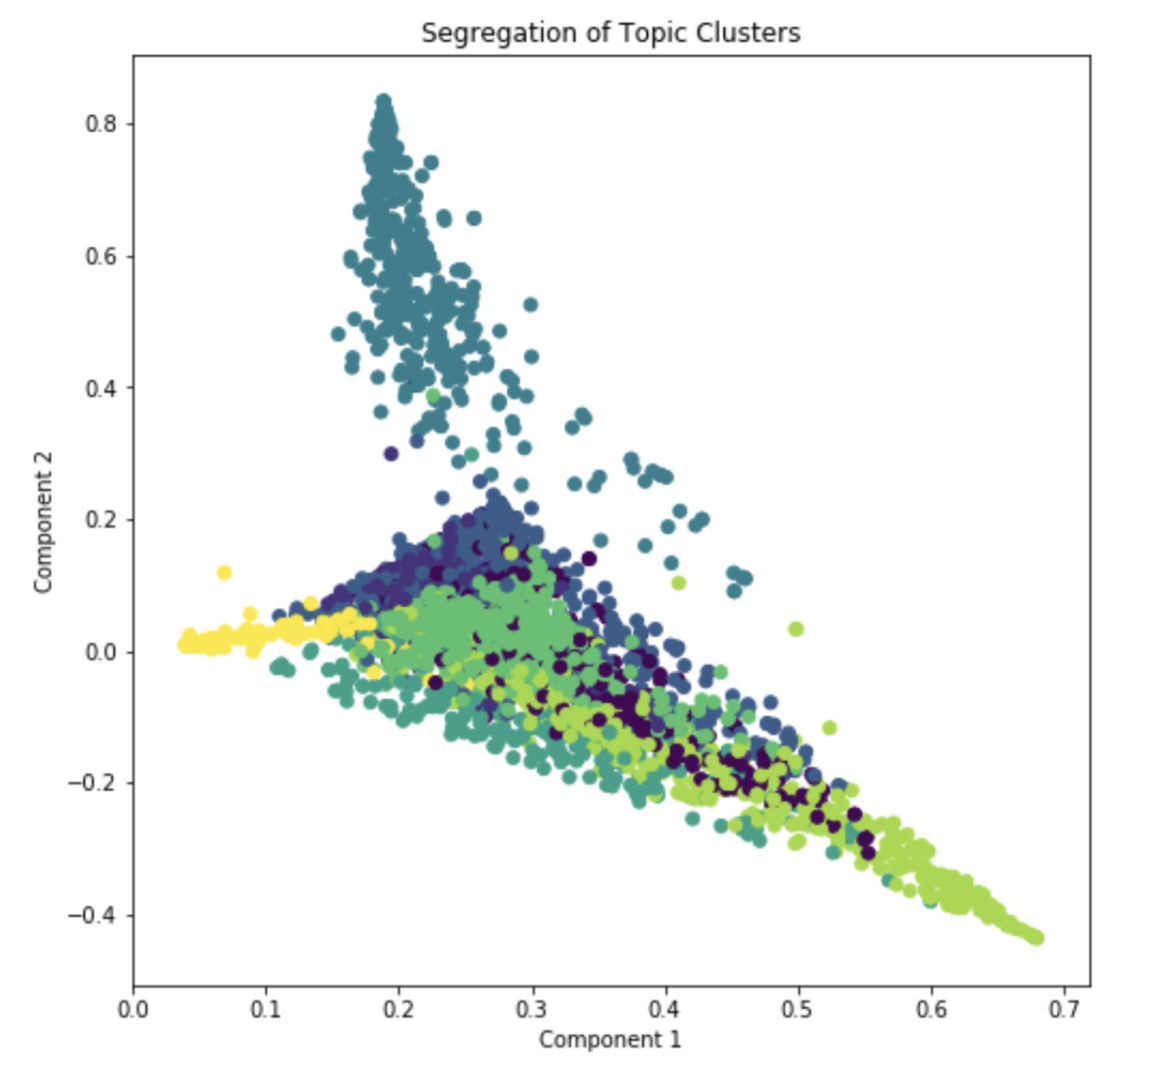
\includegraphics[width=350pt]{svd_clusters.png} \\

The first two components only capture 20\% of the variation in the data, so a 2D visualization is not great.  But it is interesting that the most clearly separately cluster (on top) corresponds to articles which are all about \textit{college} basketball as opposed to NBA basketball. Here are the 10 titles closest to the medoid of that cluster. \\

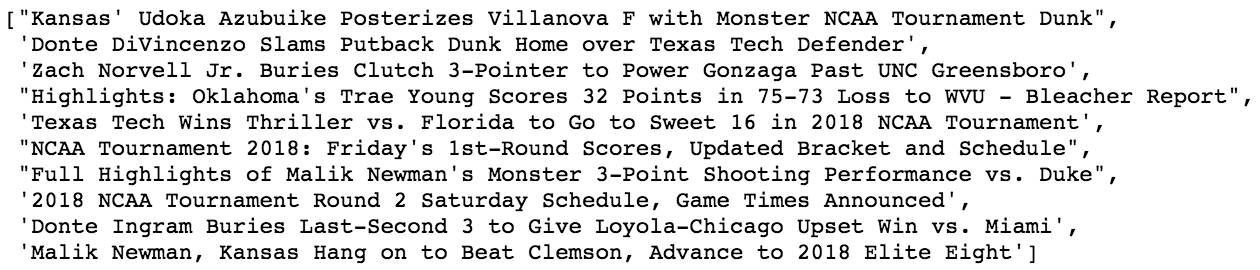
\includegraphics[width=350pt]{college_medoid_closest10.png} \\

Across the board, clustering based on the topical composition of the articles seemed to make good sense, and we felt confident in our topics. 

\section{Producing a Recommendation: An Example}
Let us see our recommender system in action.  We took a new article from May 13, 2018, entitled \textit{Keith Pompey on 76ers' Pursuit of Lebron James: Prepared to Do Whatever It Takes}, and expressed it as a distribution over the 13 topics using our trained LDA model.  Here is the distribution over topics.  We've labeled each topic according to what we think it primarily represents (as specified above and in the appendix). Not suprsingly, this article is mostly about free agency and trades. Also, notice that the topic of the 76ers is prominent. 

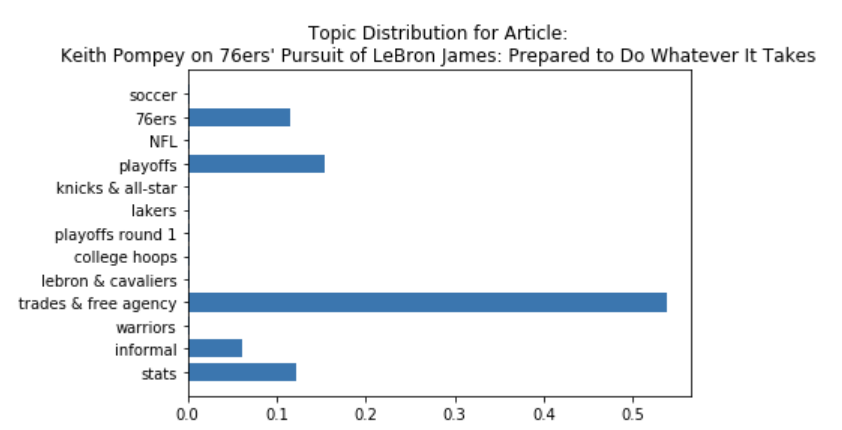
\includegraphics[width=300pt]{newarttopics.png}\\

MAKE THIS JENSEN SHANNON DISTANCE!!!!!!
MAKE THIS JENSEN SHANNON DISTANCE!!!!!!
MAKE THIS JENSEN SHANNON DISTANCE!!!!!!
MAKE THIS JENSEN SHANNON DISTANCE!!!!!!
MAKE THIS JENSEN SHANNON DISTANCE!!!!!!

Then, we found the nearest article to it using L2 norm, from all articles in the Bleacher Report corpus expressed in terms of their topic mixtures. Here's are the top 5 recommendations: \\
 
 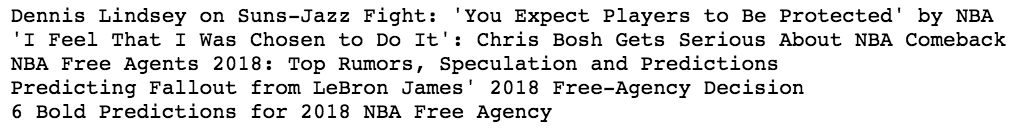
\includegraphics{preds.png}\\
 
 While some articles feel like they are not relevant (notably the first two), notice that the other three recommendations are on-point in discussing Lebron James' upcoming free agency decisions. 

\section{Discussion}
Most of the world's data is in the form of unstructured natural language, and using Natural Language Processings provides an analytics edge in many domains, not the least of which is online advertising.  It is no surprise that NLP is one of the hottest fields in research right now.  In this project we learned a lot about NLP, from data cleaning and data scraping to building topic models on a corpus of articles.  We learned a lot about three common ways of embedding documents in a vector space, and then took a deep dive into training and visualizing one of them, Topic Modeling with Latent Dirichlet Allocation. The vector-space article embedding was motivated by a desire to cluster articles to produce quality recommendations.  If hired by Bleacher Report, our first step would be to do a live test of our LDA-based recommender system.  

\section{Appendix}
\subsection{Initial Experiment to Find Most Promising Model}
\subsubsection{Word2vec}
Word2vec is a modeling approach that aims to embed words as vectors by considering their context in a corpus.  In a successful model, words that share common contexts correspond to vectors in close proximity in the space.  In our case, we with to embed \textit{articles}, not words,  so the approach we tested was to \textit{average the word embeddings in the title of the article}. 
%\subsubsection{Word2vec Pre-processing}
Word2vec training requires a set of sentences, not documents, so we began a different data-processing pipeline just for this model, starting from the scraped documents. In addition, we left in all of the words, as opposed to removing them as in the other models. The reason for this is that word2vec infers dependency information between words, and removing stop words would remove that linkage information.
%\subsubsection{Word2vec Training}
The number of word2vec dimensions is a hyperparameter that depends on the application. Most literature recommends a value of 100, and this produced very reasonable results in our case.

The closest vectors to lebron\_james are his (all-star) teammates, his hometown, his team name, and his trash-talking nemesis and other all-star rivals. \\
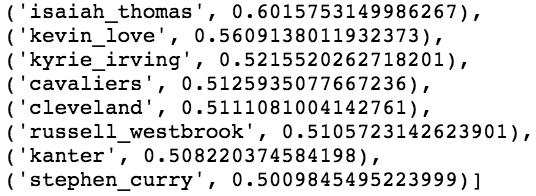
\includegraphics[width=200pt]{james_word2vec.png} 

The model correctly separates teams from the Eastern Conference from teams in the Western Conference, which you would expect from a Bleacher Report corpus with many articles about each conference separately. The model also places team mates in close proximity and can differentiate between teammates and non teammates. \\
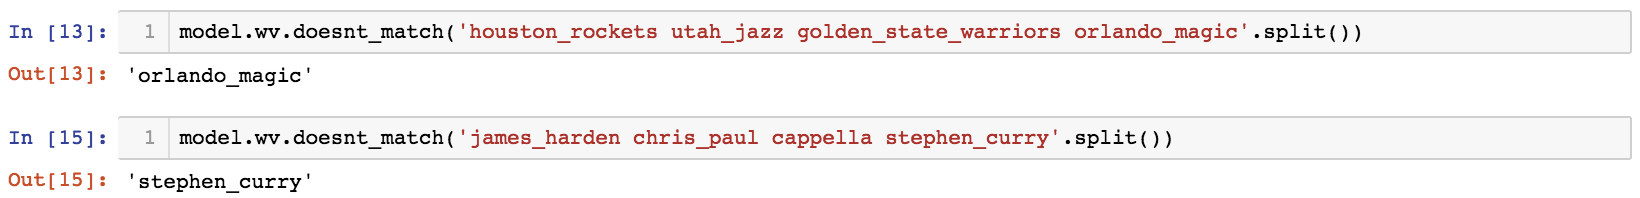
\includegraphics[width=450pt]{word2vec_diffs.png} 

\subsubsection{Non-Negative Matrix Factorization}

Non-negative matrix factorization is a group of algorithms with a strong application in recommender
systems. In our case, we will use NMF to find the underlying topics in our corpus. The mathematical
basis of NMF is quite different from LDA: basically, LDA is based on probabilistic graphical modeling
while NMF relies on linear algebra. Thus, we were curious to see which would perform better on
our corpus.

\subsubsection{Experimental Results: LDA Wins}
We applied both NMF and LDA to our corpus and eye-checked the results. At this point, our goal
was just to see if NMF would perform better than LDA, in order to choose which method to
continue with. We already found interesting packages to visualize LDA results, so
LDA was our first choice but we still wanted to check if NMF would be more suited,
though we acknowledge eye-checking might not be the most rigorous approach.
We chose to return $k=10, 13, 15, 17, 20$ topics and printed the top 10 words for each topic.
Overall, LDA returned more consistent results, while NMF would regularly return topics that 
we cannot clearly label. For example, how would we label topic 1 in the following results:

\begin{ttfamily}
 Topic 0: points game rebounds series rockets season jazz thunder games assists\\
Topic 1: nba mj triple 30 way best liangelo possiblethe clowning doublesthe\\
Topic 2: draft nfl browns lb landry app football wnba journey st\\
Topic 3: ...
\end{ttfamily}

We proceeded similaryl for word2vec and concluded we should stick to LDA.

\subsection{LDA Visualization Continued}

Topic 8 seems to capture the multiple stories around the Los Angeles Lakers this season, always a popular NBA team. 

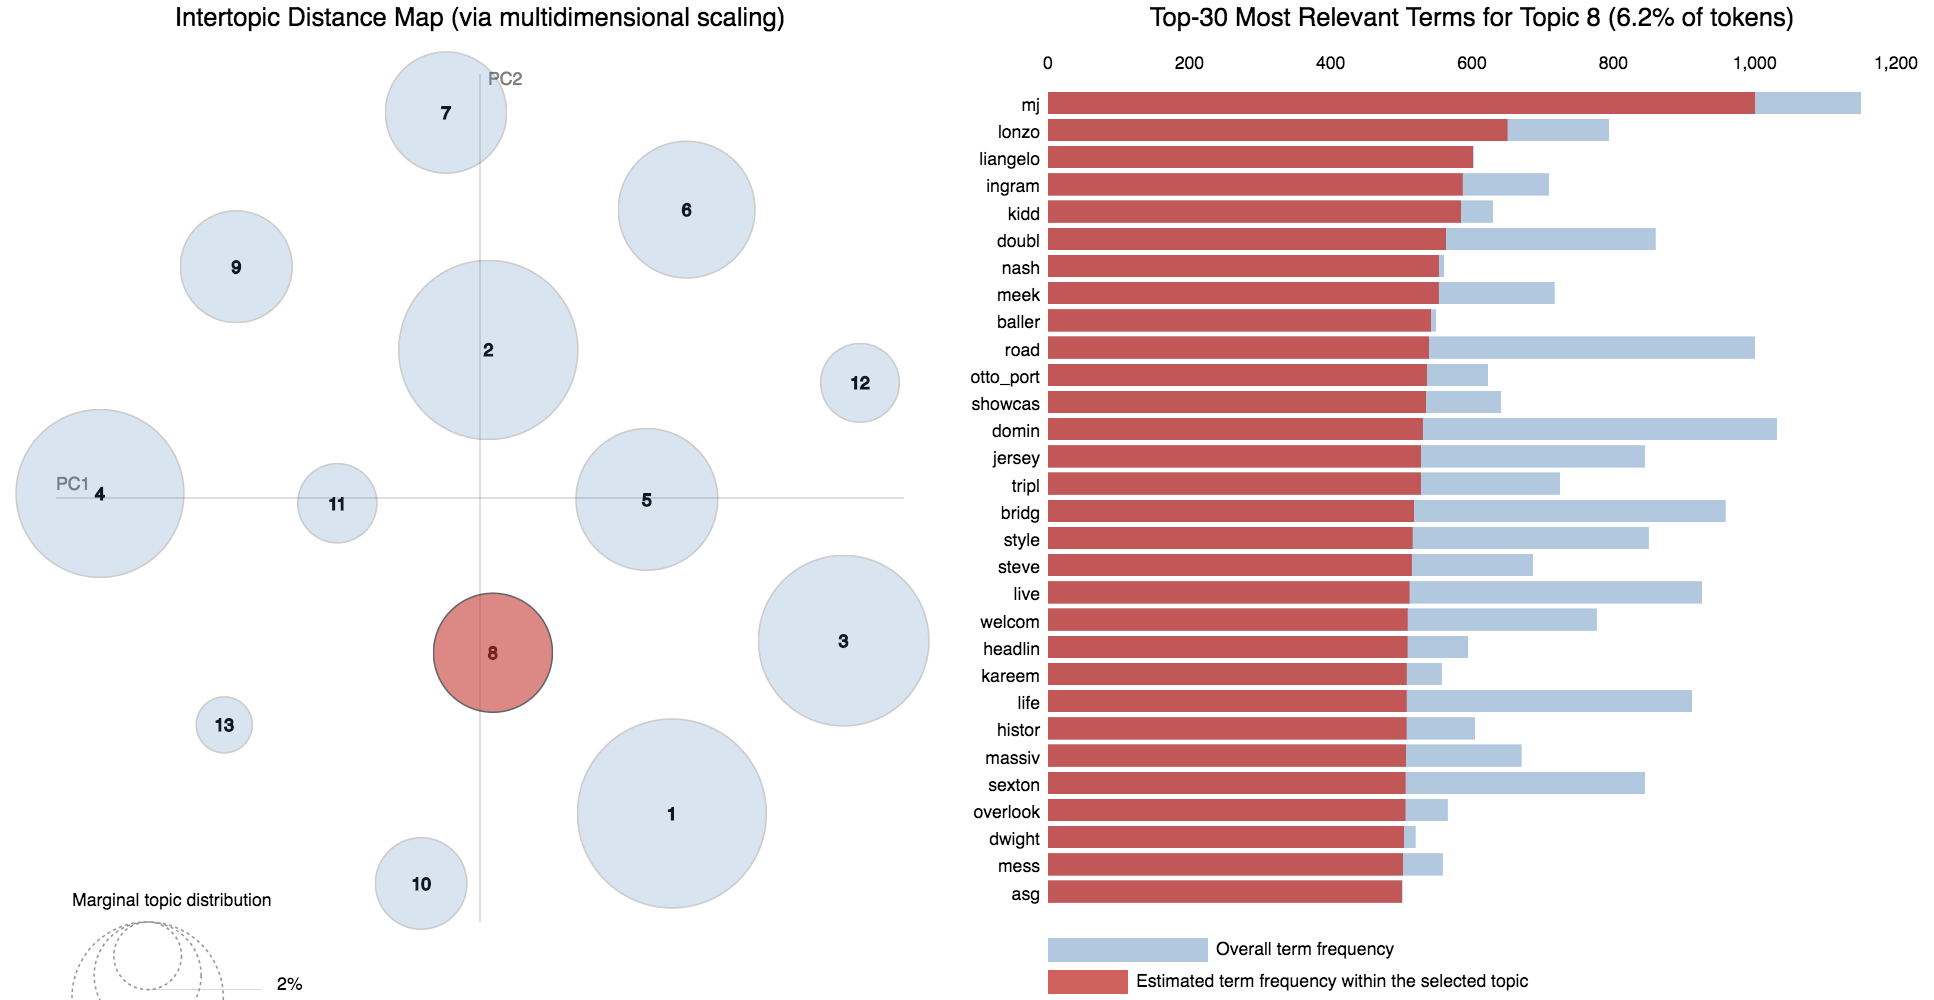
\includegraphics[width=470pt]{8.png} 

Topic 9 seems to merge two distinct topics, in our opinion - the all-star game and the New York Knicks. 

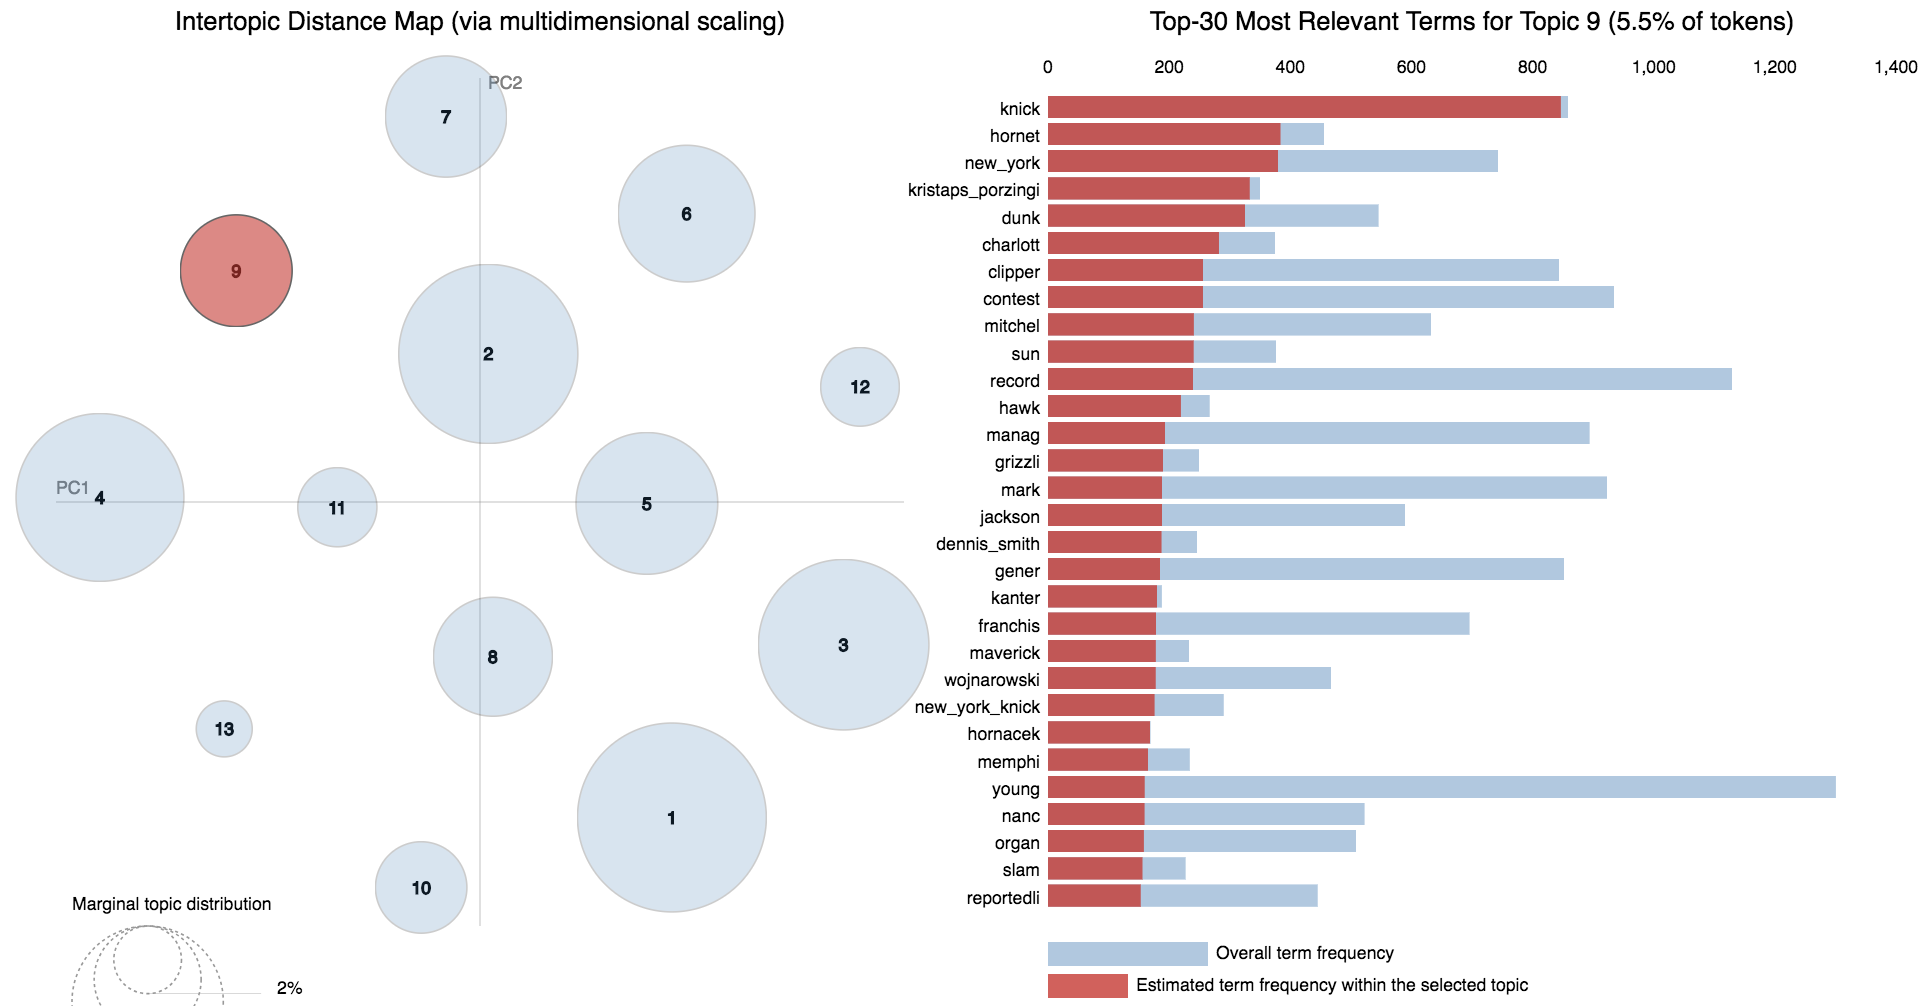
\includegraphics[width=470pt]{9.png} 

Topic 10 is about the playoffs, and includes the most notable postseason teams. 

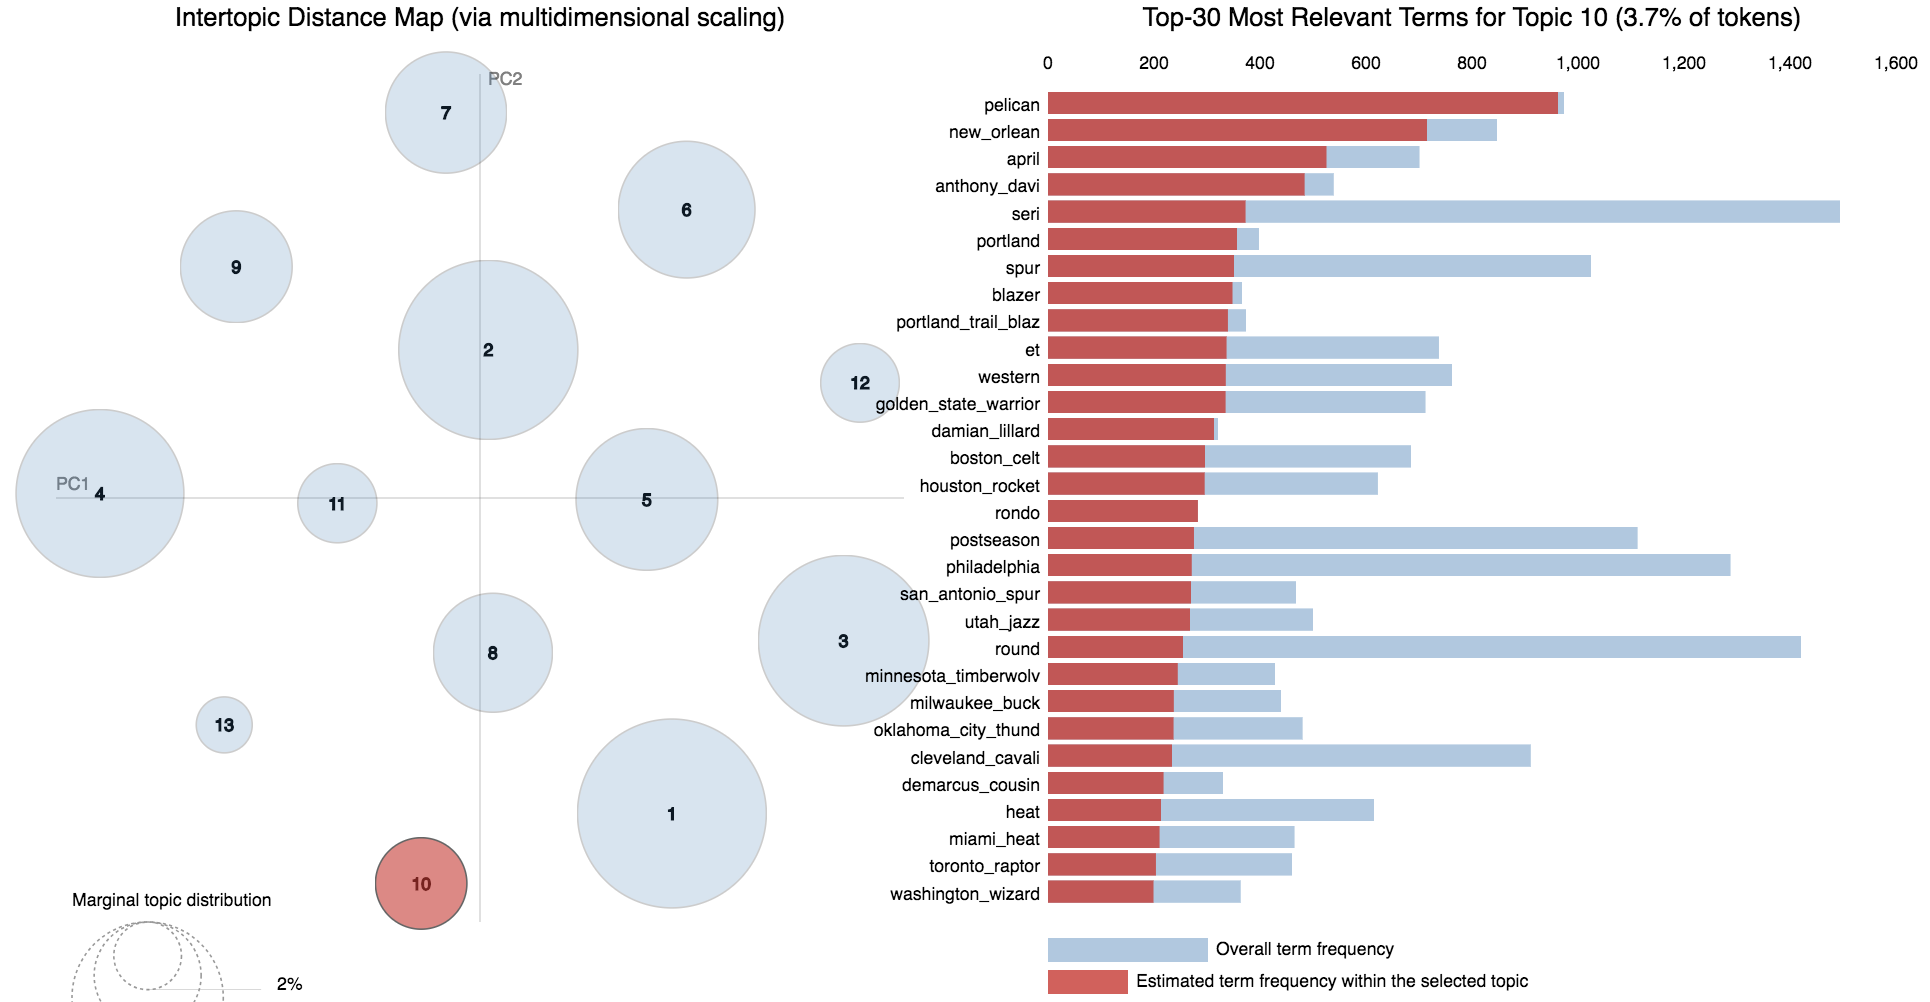
\includegraphics[width=470pt]{10.png} 

Topic 11 is actually about the National Football League!  The NewsAPI must have returned a handful of football related articles with the basketball ones, and our LDA model discovered that. 

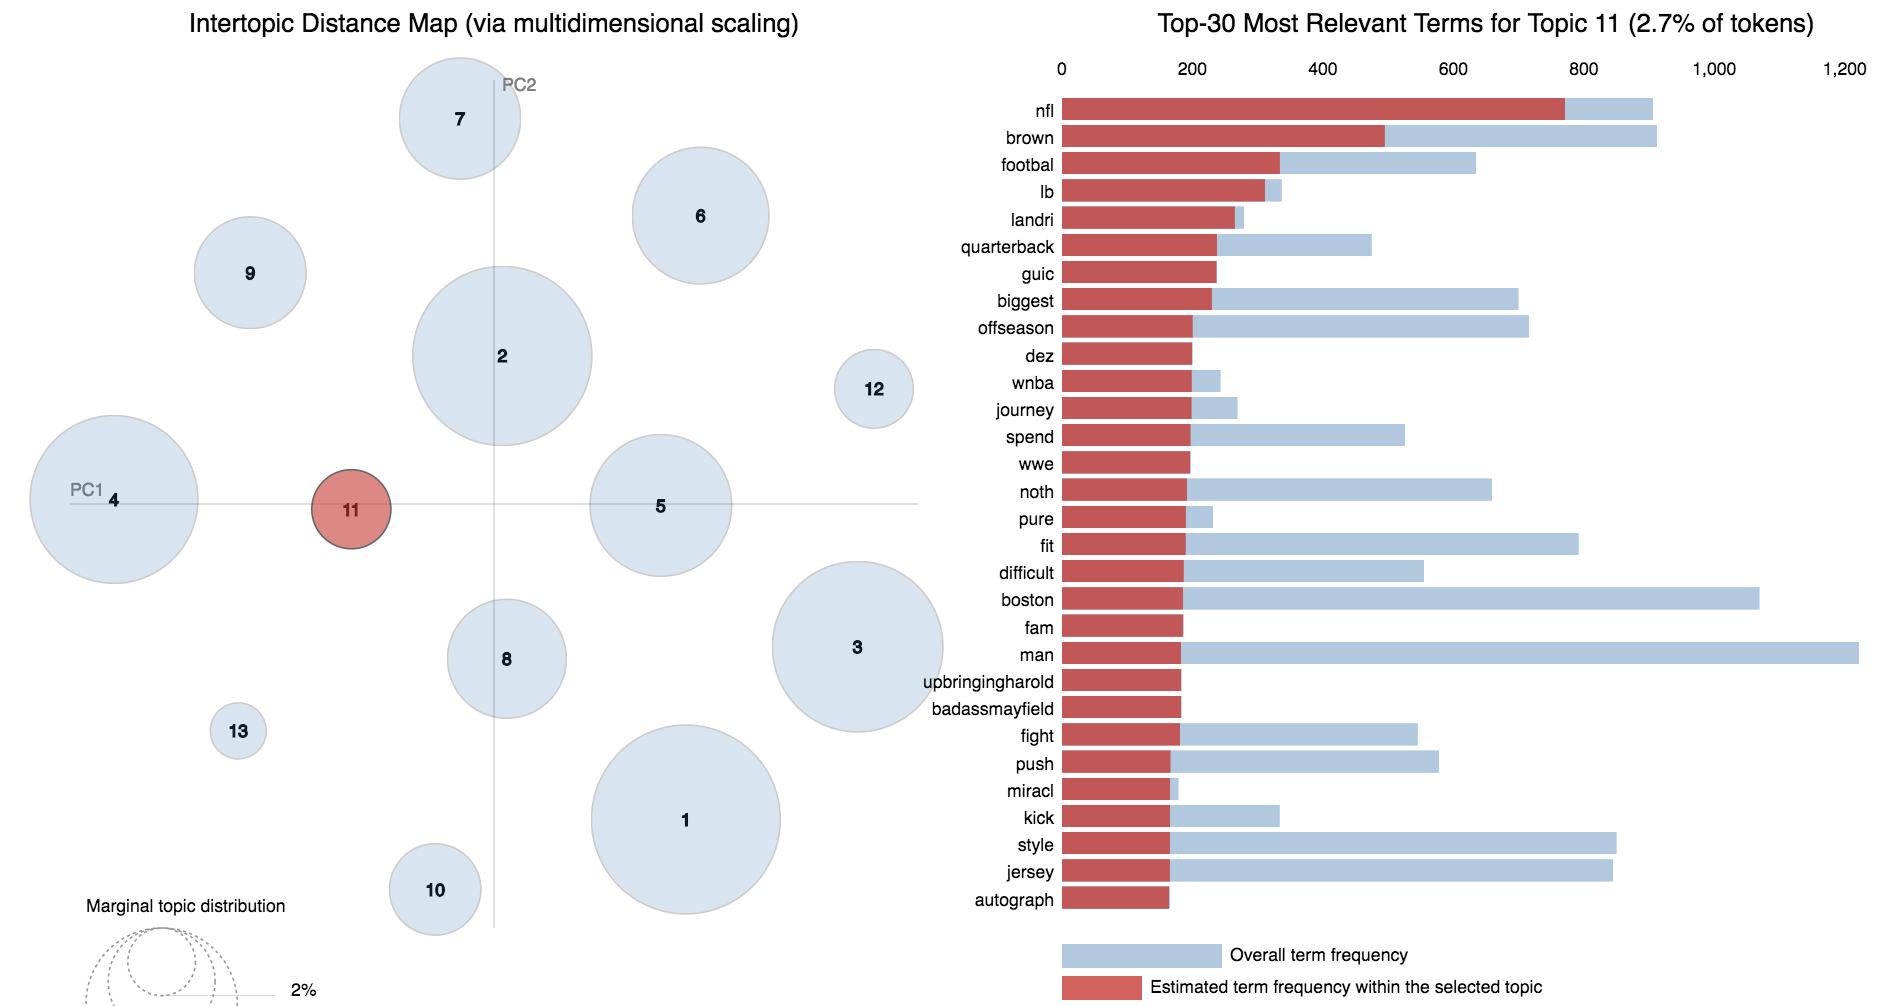
\includegraphics[width=470pt]{11.png} 

Topic 12 seems to be about the Philadelphia 76ers and their rivalry with the Miami Heat this season. The 76ers have been one of this seasons biggest sub-stories because they have two budding young superstars and are seeking to land Lebron James during free agency this summer.

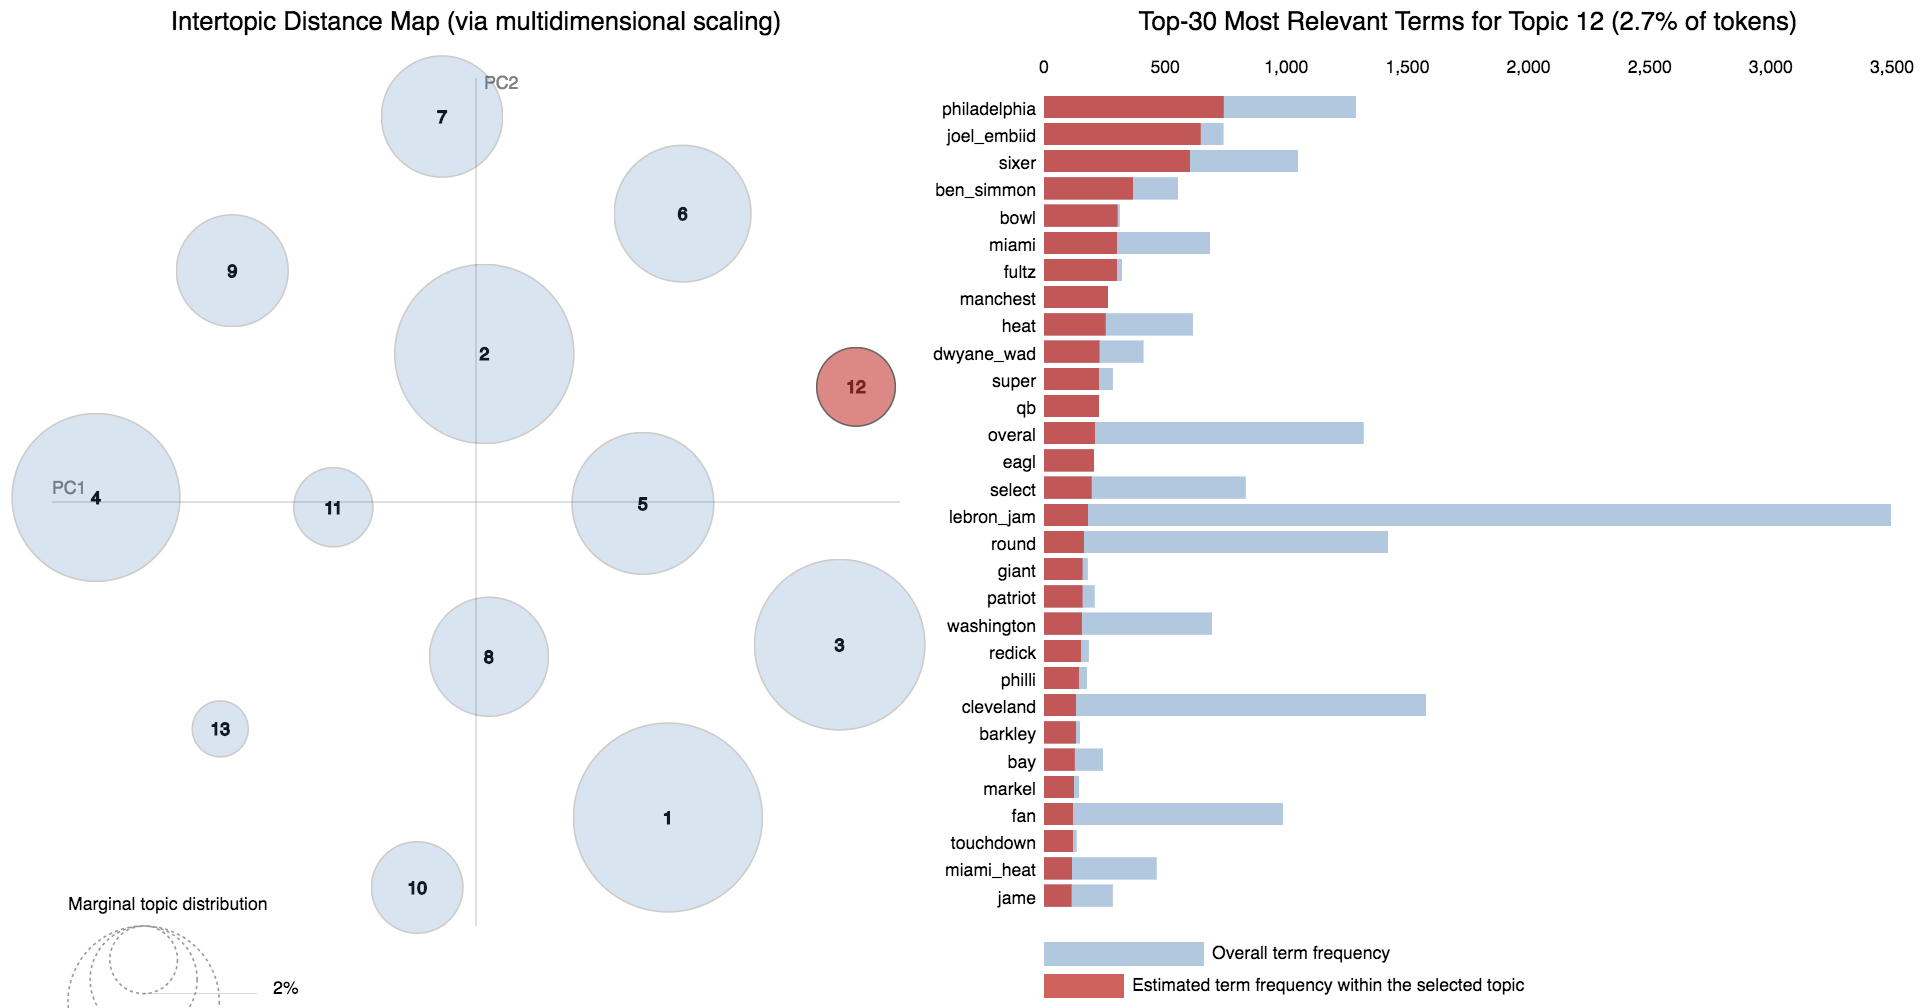
\includegraphics[width=470pt]{12.png} 

Topic 2, located in the middle of the topic clusters, seems to capture informal language. 

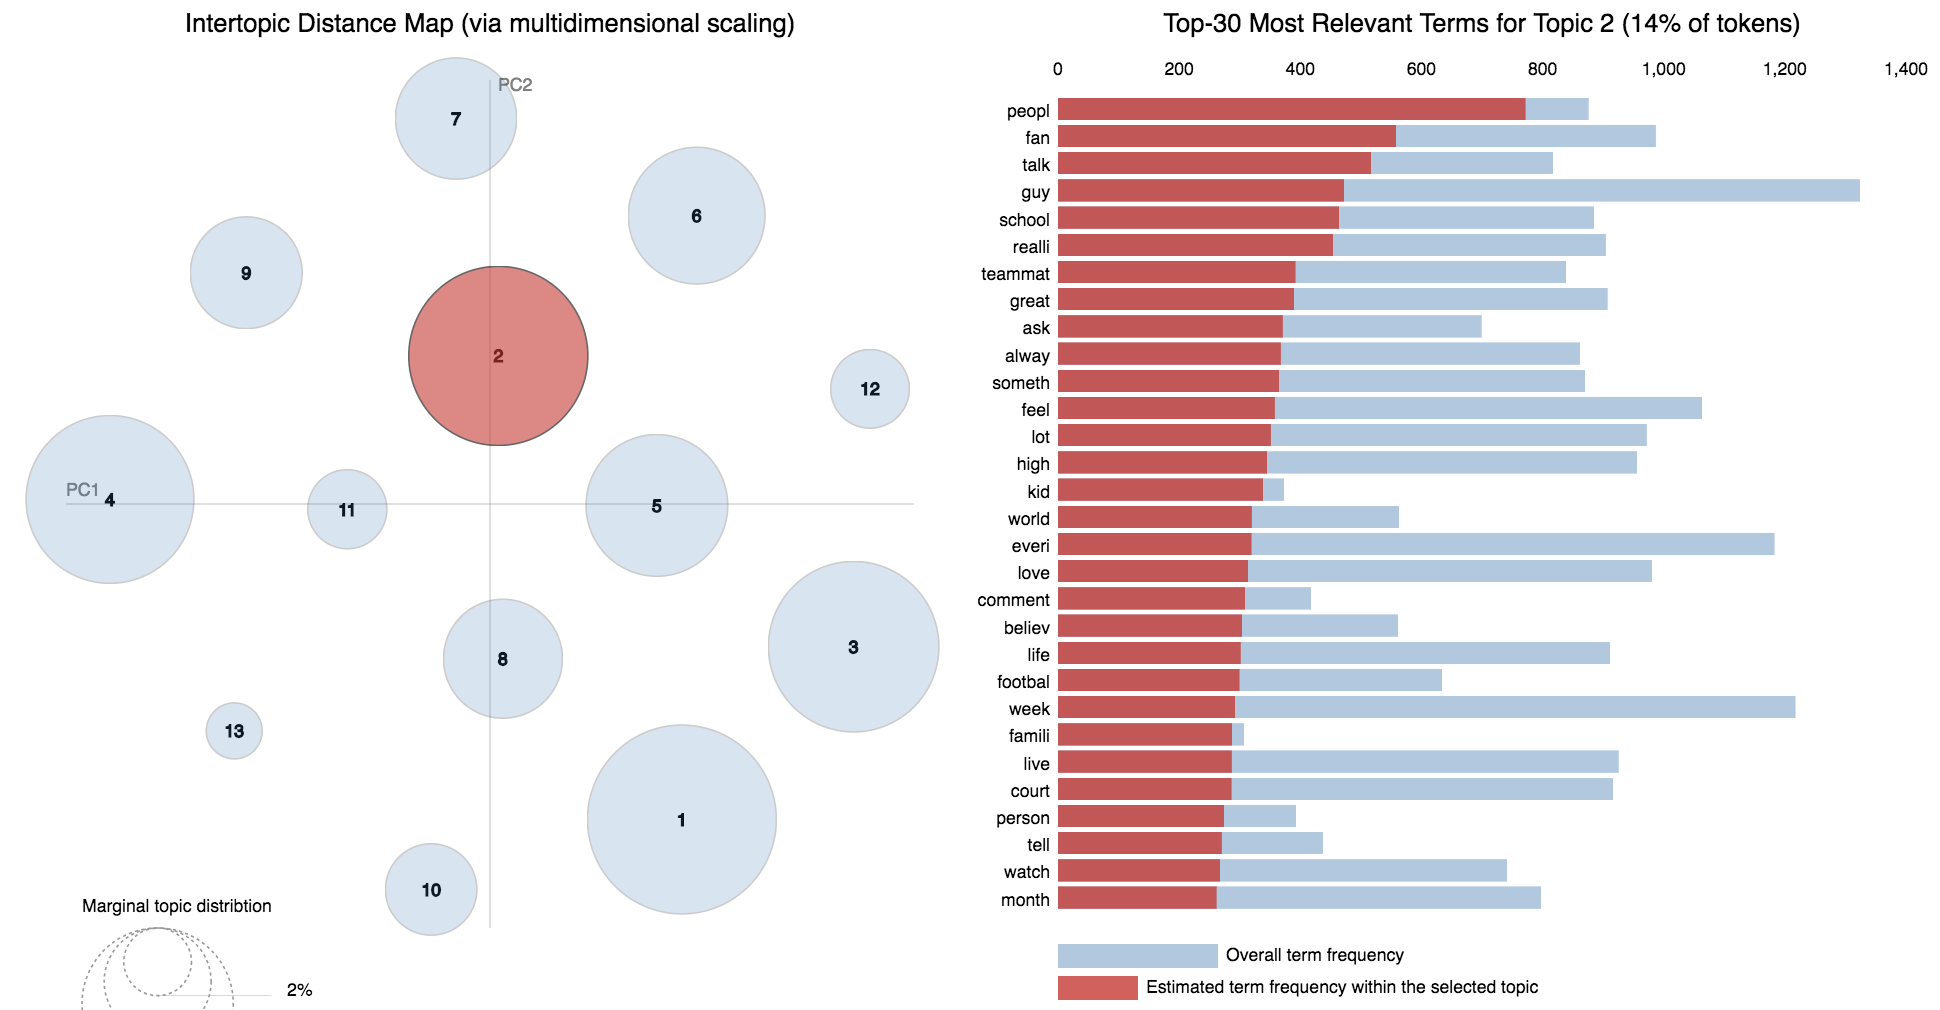
\includegraphics[width=470pt]{2.png} 



\end{document}